%% Draft document mode
\documentclass[12pt,a4paper,bibtotoc,idxtotoc,headsepline,footsepline,footexclude,BCOR12mm,DIV13]
{scrbook}

%% Final document
%\documentclass[11pt,a4paper,bibtotoc,idxtotoc,headsepline,footsepline,footexclude,BCOR20mm,DIV10]{scrbook}

% KOMA-Optionen:
%  bibtotoc: include bibliography in table of contents
%  idxtotoc: include index in table of contents
%  headsepline: use horizontalline under heading
%  BCOR: binding correcion (Bindungskorrektur) (e.g.: BCOR5mm)
%  DIV: Number of sheet sections (used for layout) (e.g.: DIV12) 

%\makeindex
	%% inter line spacing
%\linespread{1.0}

% Set here the title, authors and other stuff to be used for the cover
% This file is used by MAIN.TEX

% set title, authors and stuff for the cover
\def\doctype{Master's Thesis in Informatics}
\def\title{Smart-home intrusion detection using network intrusion detection techniques}
%\def\title{Intrusion detection on the smart-home using network intrusion detection techniques}
%\def\title{Using network intrusion detection techniques to detect intruders on the smart home}
%\def\title{Network intrusion detection techniques on the smart home domain}
\def\titleGer{Einbruchserkennung in Smart-Home Umgebungen mittels Network Intrusion Detection Techniken}
\def\author{Manuel Munoz}
\def\supervisor{Professor Bernd Bruegge, Ph.D.}
\def\advisor{Stefan Nosovi\'{c}, M.Sc.}
\def\date{November 15, 2015}

% text to appear in the footer
\def\footertext{}
var OpenHAB = {}; // Settings object


//----------- PICTOGRAM ICONS -----------
// Set "usePictogramIcons" to true if PNG pictogram icons are used. Set to false if normal color PNG images are used as icons.

OpenHAB.usePictogramIcons = false;



//----------- UPDATES -----------
// Set "enableUpdates" to "true" if you want GreenT to check for new versions and updates itself, "false" to disable updates and "password" to enable updates only after a password is provided. You can set the password via "updatesPassword" setting.

OpenHAB.enableUpdates = 'true';


// Set "updatesPassword" with your desired password (only needed when OpenHAB.enableUpdates = 'password'). 
OpenHAB.updatesPassword = '123456';
% Commands to be used within the TUM report document
% Included by MAIN.TEX
% Please include your own cool commands here. 
% Be only sure to comment it sufficiently so others can use it.

%-------------------------------------------------------------
%                      Own Commands
%-------------------------------------------------------------


%-------------------------------------------------------------
% math stuff -------------------------------------------------

% nice R, N, C
\newcommand{\nat}{\mathbb{N}}
\newcommand{\real}{\mathbb{R}}
\newcommand{\compl}{\mathbb{C}}



% norm
\newcommand{\norm}[1]{\left\| #1 \right\|}

% un demi
\newcommand{\half}{\frac{1}{2}}

% parantheses
\newcommand{\parenth}[1]{ \left( #1 \right) }
\newcommand{\bracket}[1]{ \left[ #1 \right] }
\newcommand{\accolade}[1]{ \left\{ #1 \right\} }
%\newcommand{\angle}[1]{ \left\langle  #1 \right\rangle }

% partial derivative: %#1 function, #2 which variable
% simple / single line version
\newcommand{\pardevS}[2]{ \delta_{#1} f(#2) }
% fraction version
\newcommand{\pardevF}[2]{ \frac{\partial #1}{\partial #2} }

% render vectors: 3 and 4 dimensional
\newcommand{\veciii}[3]{\left[ \begin{array}[h]{c} #1 \\ #2 \\ #3	\end{array} \right]}
\newcommand{\veciv}[4]{\left[ \begin{array}[h]{c} #1 \\ #2 \\ #3 \\ #4	\end{array} \right]}

% render matrices: 3  dimensional (arguments in row first order)
\newcommand{\matiii}[9]{\left[ \begin{array}[h]{ccc} #1 & #2 & #3 \\ #4 & #5 & #6 \\ #7 & #8 & #9	\end{array} \right]}
%DOESN'T WORK,DON'T KNOW WHY \newcommand{\mativ}[16]{\left[ \begin{array}[h]{cccc} #1 & #2 & #3 & #4 \\ #5 & #6 & #7 & #8 \\ #9 & #10 & #11 & #12 \\ #13 & #14 & #15 & #16 \end{array} \right]}


%-------------------------------------------------------------
%-------------------------------------------------------------


%-------------------------------------------------------------
% some abreviations ------------------------------------------
\newcommand{\Reg}{$^{\textregistered}$}
\newcommand{\reg}{$^{\textregistered}$ }
\newcommand{\Tm}{\texttrademark}
\newcommand{\tm}{\texttrademark~}
\newcommand {\bsl} {$\backslash$}

%-------------------------------------------------------------
%-------------------------------------------------------------


%-------------------------------------------------------------
% formating --------------------------------------------------

% Theorem & Co environments and counters
\newtheorem{theorem}{Theorem}[chapter]
\newtheorem{lemma}[theorem]{Lemma}
\newtheorem{corollary}[theorem]{Corollary}
\newtheorem{remark}[theorem]{Remark}
\newtheorem{definition}[theorem]{Definition}
\newtheorem{equat}[theorem]{Equation}
\newtheorem{example}[theorem]{Example}
\newtheorem{algorithm}[theorem]{Algorithm}

% inserting figures
\newcommand{\insertfigure}[4]{ % Filename, Caption, Label, Width percent of textwidth
	\begin{figure}[htbp]
		\begin{center}
			\includegraphics[width=#4\textwidth]{#1}
		\end{center}
		\vspace{-0.4cm}
		\caption{#2}
		\label{#3}
	\end{figure}
}




% referecing figures

\newcommand{\refFigure}[1]{ %label
	figure \ref{#1}
}
\newcommand{\refChapter}[1]{ %label
	chapter \ref{#1}
}

\newcommand{\refSection}[1]{ %label
	section \ref{#1}
}

\newcommand{\refParagraph}[1]{ %label
	paragraph \ref{#1}
}

\newcommand{\refEquation}[1]{ %label
	equation \ref{#1}
}

\newcommand{\refTable}[1]{ %label
	table \ref{#1}
}




\newcommand{\rigidTransform}[2]
{
	${}^{#2}\!\mathbf{H}_{#1}$
}

%code, in typewriter
\newcommand{\code}[1]
 {\texttt{#1}}

% comment that appears on the border - very practical !!!
\newcommand{\comment}[1]{\marginpar{\raggedright \noindent \footnotesize {\sl #1} }}

% page clearing
\newcommand{\clearemptydoublepage}{%
  \ifthenelse{\boolean{@twoside}}{\newpage{\pagestyle{empty}\cleardoublepage}}%
  {\clearpage}}


%-------------------------------------------------------------
%-------------------------------------------------------------


\newcommand{\etAl}{\emph{et al.}\mbox{ }}

\makeglossary

\begin{document}

	\frontmatter
	% The front cover for the TUM report document.
% Included by MAIN.TEX


%--------------------------------------------------
% The Front Cover
%--------------------------------------------------

% The front cover for the TUM document.
% Included by MAIN.TEX


%--------------------------------------------------
% The Front Cover
%--------------------------------------------------

% correct BCOR - undo at the end !!!
\def\bcorcor{0.15cm}
\addtolength{\hoffset}{\bcorcor}

\thispagestyle{empty}

 \vspace{4cm}
\begin{center}
	       \oTUM{4cm}
	   
	   \vspace{5mm}     
	   \huge FAKULT{\"A}T F{\"U}R INFORMATIK\\ 
	   \vspace{0.5cm}
	 \large DER TECHNISCHEN UNIVERSIT{\"A}T M{\"U}NCHEN\\
    \vspace{1mm}
        
	\end{center}
		

\vspace{15mm}
\begin{center}

   {\Large \doctype}

  \vspace{20mm}
  
  {\huge\bf \title}\\%[3ex]
  
    \vspace{15mm}
  
  
  {\LARGE  \author}
  
  \vspace{10mm}
  
  \begin{figure}[h!]
  \centering
   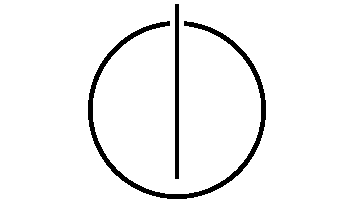
\includegraphics[width=4cm]{styles/informat.png}
  \end{figure}
  
  \end{center}
	\clearemptydoublepage
	% The titlepage for the CAMP report document.
% Included by MAIN.TEX


%--------------------------------------------------
% The title page
%--------------------------------------------------

% correct BCOR - undo at the end !!!
\def\bcorcor{0.15cm}
\addtolength{\hoffset}{\bcorcor}

\thispagestyle{empty}

 \vspace{10mm}
\begin{center}
	       \oTUM{4cm}
	   
	   \vspace{5mm}     
	   \huge FAKULT{\"A}T F{\"U}R INFORMATIK\\ 
	   \vspace{0.5cm}
	 \large DER TECHNISCHEN UNIVERSIT{\"A}T M{\"U}NCHEN\\
        
	\end{center}
		

\vspace{10mm}
\begin{center}

   {\Large \doctype}

  \vspace{10mm}
  
  {\LARGE \title}\\
  
  
  \vspace{10mm}
  
  
  {\LARGE  \titleGer}\\
  
  
  \vspace{10mm}

    %\hfill
    \begin{tabular}{ll}
	   \Large Author:     & \Large \author \\[2mm]
	   \Large Supervisor:    & \Large \supervisor \\[2mm]				
	   \Large Advisor:	& \Large \advisor \\[2mm]
	   \Large Date:       & \Large October 30, 2013
	 \end{tabular}
	 
	 \vspace{5mm}
	 
	 \begin{figure}[h!]
  \centering
   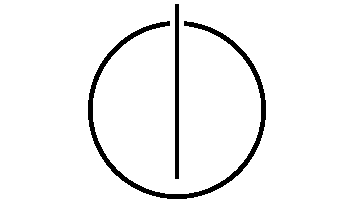
\includegraphics[width=4cm]{styles/informat.png}
  \end{figure}
   

\end{center}

% undo BCOR correction
\addtolength{\hoffset}{\bcorcor}
	\clearemptydoublepage


\thispagestyle{empty}
	\vspace*{0.8\textheight}
	\noindent
	
	I assure the single handed composition of this master's thesis only supported by declared resources.
	
	\vspace{15mm}
	\noindent
	Munich, Germany, 2013-10-31 \hspace{5cm} \author
\newpage
	\clearemptydoublepage
\phantomsection
\addcontentsline{toc}{chapter}{Acknowledgements}	


%\chapter*{Acknowledgements}

\vspace*{2cm}

\begin{center}
{\Large \bf Acknowledgments}
\end{center}

\vspace{1cm}


Many have sported me one way or the other to while writing these thesis. If I fail to mention your name, it is does not represent how grateful and lucky I am for having your support. 

I would specially like to thank my adviser Stefan Nosovi\'{c}. His constant support, encouragement, and willingness to discuss ideas greatly helped me during the process of writing my thesis. I also would like to thank Professor Bernd Bruegge for the chance to develop this work in the chair of the university that I believe to be the coolest. Furthermore, his feedback greatly enhanced my understanding of the problem at hand.

I also would like to thank my family in my mother tongue. If you do not understand Spanish, please do not take it personally. The gist of it is that they are awesome and I could not be here without them.\\
A mi familia muchas gracias por todo el apoyo que me han brindado desde la distancia. Sus constantes palabras de \'{a}nimo y sobretodo su ejemplo de perseverancia, han influido mucho la persona que soy hoy en d\'{i}a. 

	% Abstract for the TUM report document
% Included by MAIN.TEX


\clearemptydoublepage
\phantomsection
\addcontentsline{toc}{chapter}{Abstract}	

\vspace*{2cm}
\begin{center}
{\Large \bf Abstract}
\end{center}
\vspace{1cm}


In recent years we have witnessed increasing interest in smart environment from researches, and from the public, about smart homes. The appliance industry has noted this interest and also has increased the number of products geared towards home automation.
These products take advantage of wireless communication technologies to monitor, and in some cases autonomously control the environment they are in. Through their interaction and collaboration, they can make spaces more comfortable and more secure. Nevertheless, the alternatives for smart home security are not yet appealing. In order to be attractive to the general consumer, they have to outperform the traditional security systems. 

One of the problems facing traditional home security systems, is the issue of false positives. A false positive, in the context of the home, is defined as reporting an intrusion or a burglary when really nothing has occurred. We developed a system that aims to reduce the occurrence of false positives, while detecting security anomalies. To that effect, we explored the available research and existing algorithms from the networking discipline, which has dealt with intrusion detection since the 1960s. 

We aim to address these issues with the development of Rosie, a system that collects and analyses data from sensors, in order to recognize usual behavior of the inhabitants of the home, and distinguish it from abnormal behavior. 

Rosie, also serves as a platform for studying new intrusion detection algorithms, by providing simple ways of extending the software. As a proof of concept, the system uses algorithms from network intrusion detection systems. These techniques analyze communication, temporal patterns of the network traffic loads, and the content of the packets. The same type of information can be found in smart environments, and is therefore useful for distinguishing usual and unusual behavior of inhabitants.


	\tableofcontents
  	\clearemptydoublepage

\phantomsection
\addcontentsline{toc}{chapter}{Outline of the Thesis}

\begin{center}
	\huge{Outline of the Thesis}
\end{center}

%--------------------------------------------------------------------

\noindent {\scshape Chapter 1: Introduction}  \vspace{1mm}

\noindent  The introduction starts with a motivation by describing the current challenges of ... \\

\noindent {\scshape Chapter 2: Requirements Elicitation}  \vspace{1mm}

\noindent  Chapter 2 describes the requirements elicitation which includes the scenarios that drive the development of this project. Based on these scenarios, non-functional requirements are proposed and a functional model with use cases and functional requirements is elaborated. \\

\noindent {\scshape Chapter 3: Analysis}  \vspace{1mm}

\noindent  Chapter 3 describes an analysis model based on the requirements. The model is created to formalize the objects and information that exist in the domain of ... \\

\noindent {\scshape Chapter 4: System Design}  \vspace{1mm}

\noindent  Chapter 4 describes the system design model which contains ... \\

\noindent {\scshape Chapter 5: Object Design}  \vspace{1mm}

\noindent Chapter 5 describes ...
Afterwards, the transformation of application domain objects to solution domain objects is discussed. \\

\noindent {\scshape Chapter 6: Conclusion}  \vspace{1mm}

\noindent  Chapter 6 concludes with an overview of the results. Afterwards, the results are reviewed critically and visions for future work are pointed out. \\


	
% ---------------------------------------------------------------------------
%
% 	Thesis Main Part
%
% ---------------------------------------------------------------------------

\mainmatter
\chapter{Introduction}
\label{chapter:Introduction}
In recent years the we have witnessed increasing interest in smart environment research \cite{1010072F1159031611}. This trend has also been followed by the interest of users about smart homes \cite{googletrends}. The number of products geared towards home automation has increased, which can be seen from the amount of attention these products attract at trade shows like CES \cite{cnet} and IFA \cite{cnetIFA}, and the increasing coverage by the media, where they have become the main attraction. \\
Big manufacturers of consumer electronics reacted to this trend, and launched product lines aimed towards the home market segment, making home automation not longer restricted to enthusiasts.\\
These products take advantage of wireless communication technologies to monitor, and in some cases autonomously control the environment they are in. Through their interaction and collaboration they can make spaces more comfortable and more secure. However, for a smart home security alternative to be appealing to the general consumer, it has to outperform traditional security systems. 

\section{Problem Statement}
One of the problems facing traditional home security systems, is the issue of false positives. In terms of home security, a false positive is defined as reporting an intrusion or a burglary when really nothing has occurred. According to Blackstone \etAl \cite{Blackstone2005233}, one of the larger issues that negatively impact on communities, is the elevated frequency in which first responders have to attend and investigate false alarms. Specifically, Blackstone \etAl claim that the response to burglar alarms by police officers amount from 10 to 20\% of all the received calls. However, more disconcerting is the fact that 94 to 99\% of those calls are false alarms. \\
Some cities and municipalities try to counteract this problem by imposing fines \cite{Blackstone2005233}, which can be as high as \$1000 USD for repeating offenders. In some cases, legal action has also be taken \cite{Blackstone2005233}. Some users were charged and convicted for offenses that are subject to a mandatory prison time. However, the highest burden of a high frequency false positive rate impacts the whole neighborhood. Concretely, Blackstone \etAl assert that in such areas police tend to lower the priority of those calls, directly affecting the "deterrence effect" of owning an alarm system \cite{Blackstone2005233}. 
\\
\section{Proposed Solution}
To tackle many of these issues, we take advantage of the increasing popularity and decreasing prices of home sensing equipment. We developed a system that aims to reduce the occurrence of false positives. To that effect, we explored the available research and existing algorithms from the networking discipline, which has dealt with intrusion detection since the 1960s. Our goal is to take the advantages of machine learning algorithms for network intrusion detection and applying them to the smart home domain.


\section{Related Work}
\label{related_work}

%The Aware Home, Georgia Tech University
\textbf{Kidd \etAl, 1999: The Aware Home: A Living Laboratory for Ubiquitous Computing Research \cite{raey}} \\
The Aware Home is a project from the Georgia Institute of Technology. It was created as "a living laboratory for interdisciplinary design, development and evaluation" \cite{Kientz:2008:GTA:1358628.1358911}. The objective of the project was to provide a platform where different disciplines could test their hypotheses regarding new technologies for the smart home. The team at the Georgia Institute of Technology built a three-story house and equipped it with sensors that captured and registered almost every event that happened around the house, using pinhole cameras, microphones, voltmeters, etc. Applications that where developed for this context, target specific scenarios like supporting aging in place, and supporting busy families. \\
The first scenario addresses problems that stay-at-home senior citizens may have. Issues such as safety, accident prevention and detection, aid in daily activities (reminders and familiarization with new technologies), and facilitating communication with the outside. For example, the project \textbf{Memory Mirror} \cite{Kientz:2008:GTA:1358628.1358911} identifies objects used by the resident, and posts them on a mirror creating a reminder. In the case the user has interacted with the object before, the mirror posts usage statistics.
The second scenario, supporting busy families, targets households where parents work but also need to take care of another family member. The issues include home schedule maintenance, care for individuals with special needs, and making life more enjoyable. The \textbf{Baby Steps} \cite{Kientz:2007:GKU:1240624.1240830} project tracks and logs milestones on the baby's cognitive development cycle. That way, if a milestone is missed, the house itself can provide additional timeline information to the doctors.\\
This project from the Georgia Institute of Technology is a good example of what it can be done, when a living space is designed and built from the ground up as a smart space. The house was planned from the start to have a large set of sensors. For example, for activity recognition the Aware Home has 10 pin-hole cameras in just one room \cite{Kientz:2008:GTA:1358628.1358911}. \\
Our project is focused on living spaces that already exist, and it is not possible to install a high number of sensors.\\
From the applications point of view, none of the Aware Home projects tackle the problem of home security or intrusion detection. However, it supports the use of machine learning algorithms for activity identification in a home environment, which its use is an important assumption made by our research. \\

%MavHome, University of Texas at Arlington
\textbf{Cook \etAl, 2004: MavHome: An Agent-Based Smart Home} \cite{1192783} \\
The University of Texas at Arlington proposed an architecture to model the home as a rational agent. It uses sensors to measure what happens in a home, and through different actuators the system acts on the home, altering its state. MavHome proposes an architecture that allows the home to learn the behavior of the inhabitants and interactions they have with the home. The agent uses a layered architecture \cite{1192783} with four layers. The physical layer communicates the system with the hardware components of the house. The communication layer transmits the data between agents. The information layer is responsible to gather, store, and generate new knowledge that is going to be used on the decision-making process. The decision layer takes the knowledge provided by the information layer and selects actions to be executed. The decision layer uses prediction algorithms to take sequences of interactions between the inhabitant and the home, and then compares them with previously stored sequences in order to predict the next possible actions. However, the events that can be automated are the ones that occur with a certain frequency. \\
To test the project the university also built two physical spaces and a simulation space \cite{inhabitantguidanceofsmartenvironments}. The first physical space, is a workplace environment equipped with work areas, cubicles, a break room, a lounge, and a conference room. The second space is completely equipped apartment. The project also counts with a simulation tool that allows the machine learning algorithms to be trained, to be later deployed on the physical environments.\\ 
The project arrived at one conclusion that is of importance to our project. Machine learning algorithms can be used to "model and predict inhabitant activities, and that a policy can be learned using this information to automate a smart environment" \cite{inhabitantguidanceofsmartenvironments}. Furthermore, the division of responsibilities using a layered architecture, where each layer processes the information from the previous layer, and builds upon it to then be served to the next layer, is interesting and can be explored in the context of this work.\\

%The Adaptive House, University of Colorado at Boulder
\textbf{Mozer, 2004: Lessons From An Adaptive House} \cite{mozer2004lessons} \\
The Adaptive Home is a project for the University of Colorado at Boulder. It started 1996, with the idea that smart homes should not provide a different control interface from the one that users normally use. The house uses machine learning algorithms to control different systems like heating, ventilation, air conditioning, the water heater, and lighting. The Adaptive Home, after observing the interaction between the house and the users, can deduct patterns and make predictions. If the users are not happy with the predictions, they can change the values selected by the house using the normal interface. The main objective of the Adaptive Home is comfort while reducing operating costs \cite{mozer2004lessons}.\\
The algorithm uses two constraints that need to be optimally satisfied: cost and discomfort. Through reinforcement learning, it is possible to calculate the next action for the current state, or for the next predicted state. Coarse activity identification is also one of the main focuses on the project. Once an activity is identified, the system can trigger an event that in turn will change the state of the house into the predicted one \cite{mozer2004lessons}.\\
This project not only boosts the idea from using machine learning in the home environment, but also provides an interesting perspective to that aspect, because it includes the discomfort constraint. The system calculates the cost of performing an action not only in monetary value, but also with how annoying the action can be if it is wrong. It is also interesting that it does not discretized time into timed intervals, but into event changes that trigger states changes.\\
For this project, security of the smart home was not explored. However, the use of machine learning algorithms supports the idea that it is possible to do activity identification. Furthermore, it ratifies that the environment of a smart home can be condensed on a set of predefined states, and execute actions according to those states.  If this idea is adapted to the security domain, it is possible to define the threat level of the home as states, and in turn execute actions accordingly.\\

%Aire project: Focuses on work spaces

%CyberManor, Internet Home Alliance. Company, not a Uni project
%CASAS Smart home project. Data sets MavHome comes from them.
%EasyLiving, Microsoft
%Hal, MIT Artificial Intelligence Laboratory. No home automation project
%Home Automation, IBM

%House_n, MIT
\textbf{Intille, 2004: The Goal: Smart People, Not Smart Homes} \cite{smartpeople} \\
The Massachusetts Institute of Technology also conducted research in the field of the smart home with a multi-disciplinary approach. Many industry partners and other departments at MIT co-founded the House\underline{ }n project. The goal of this project \cite{smartpeople} was to shift the investigation's focus from a smart home that automates all possible activities, to one where the smart home requires user's interaction to help maintaining life stimulating \cite{smartpeople}.\\
Within the House\underline{ }n project, MIT joined forces with industry partners and used the approach of building a live-in laboratory. There, volunteers would move in for a period of time and lead their lives normally, and allow to measure their activities by sensors. The laboratory was built in 2004 and it is called the PlaceLab \cite{placelab}. 
The focus of this project was proactive health care \cite{placelab}. By providing relevant, just-in-time information, the home influences the occupants to make better dietary choices. Also, the project focuses on the influence of how technology can impact independence of aging seniors \cite{aginginplace}, using different methods of indoor positioning \cite{bhack}, and the implications of user tracking \cite{info:doi/10.2196/jmir.8.4.e29}. All other projects tackled problems from other disciplines like material engineering and architecture.\\
%IIB, Trinity College Dublin
%i-LAND, Ambiente
%Interactive Workspaces, Stanford University. collaborative work settings
%Neural network house from 1995. May be too old.
%PRIMA, Inria
%The intelligent home 1999. May be too old.
%Smart Spaces Lab, NIST. Project for working spaces detecting meetigns 
%SMART Connected Home, GE

%Machine learning
\textbf{Fung \etAl, 2013: Intrusion Detection Networks: A Key to Distributed Security} \cite{fung2013CRC} \\
Intrusion detection systems are designed to monitor all elements deployed in a network, and alert in case out of the ordinary behavior is detected. Network intrusion detection techniques can be divided into the following two methods: Signature-based and anomaly-based \cite{fung2013CRC}. Signature-based techniques use a predefined list of already identified intrusion methods, and compares the network's traffic to filter out possible intrusion attempts. Anomaly-based techniques compare the behavior of the network with a precollected baseline of normal behavior \cite{fung2013CRC}. This technique is the one we want to explore with our current work, under which circumstances anomaly detection can be extended to the smart environment, and which of the intrusion detection methods can be also used in the home.\\
 
\textbf{Bhattacharyya \etAl, 2013: Network Anomaly Detection: A Machine Learning Perspective \cite{Bhattacharyya:2013:NAD:2505468}} \\
The work of Bhattacharyya \etAl analyzes the different machine learning techniques used on anomaly-based network intrusion detection. According to the authors, it is possible to analyze the traffic on a network and then classify it between malicious or normal behavior. This characteristic turns the anomaly detection problem into a classification problem \cite{Bhattacharyya:2013:NAD:2505468}, as specified below: \\
%The authors also present a list of requirements that must be met by real-time or near real-time systems, that can be adapted to the smart home environment:
\begin{enumerate}
	\item These systems must detect anomalies with high detection accuracy with minimal or even no prior knowledge of the environment, and also must observe the environment and learn what is the normal behavior. 
	\item The identification process must be done with the minimum amount of false positives. 
	\item The number of features should be the least possible. The authors also propose other two requirements, which are already implicit to the smart environment.
\end{enumerate}
The work of Bhattacharyya \etAl also categorizes the machine learning techniques used for network anomaly detection into six categories, from which we describe four that are most relevant for our problem: 
	\begin{itemize}
		\item \textbf{Supervised learning}
		
This method assumes that it is possible to start with a batch of labeled data, called a "training set". This collection of data is used to build a model, to which all new data can be compared against and decide if the behavior is normal or not. This categorization is divided into parametric and nonparametric methods. \\
The first approach assumes that the data is produced using a parametric distribution and probability density function.
The second approach, the nonparametric method, does not start with a model, but creates one from the data. The most used nonparametric method for anomaly detection is to take the training set and create a function that maps sample data to the interval from [0,1]. Then, a data point is evaluated with that function. If it scores under a certain predefined threshold is considered anomalous.\\
One of the advantages of using supervised learning, is that if the system runs for a certain amount of time, it is possible to establish a very good baseline to be used as a comparison. The disadvantages include susceptibility to being trained to consider malicious traffic as normal. Also, due to the assumptions made by the model, and on the grounds that setting all the parameters is very difficult, the ratio between false positives and false negatives is unfavorable.\\

		\item \textbf{Unsupervised learning}
		
For supervised learning it is very important to have labeled data. Nevertheless, obtaining that data may be very difficult or expensive, since the use of experts is needed. Methods that do not rely on labels are called unsupervised, and they may be better suited to set the baseline that represents normal behavior. \\

One of the methods is \textit{clustering}. Here a representative point is selected for each desired cluster, then each test data point is taken, and classified according to the nearest cluster. Here the disadvantage of an expert becomes again apparent. Nevertheless, works like UNADA \cite{unada} where Casas \etAl{} introduced a clustering algorithm for unsupervised network anomaly knowledge-independent detection of anomalous traffic. 

This algorithm uses a clustering technique to identify clusters and outliers in multiple low-dimensional spaces.\\

%needs explanation of how it works and how it can be translated to smart homes
\textit{Association mining} tries to identify events that occur simultaneously. This technique assumes that patterns in the data can be identified. Typical usage of association mining is, when stores perform market research to better stock their shelves. Analyzing the data it is possible to come interesting conclusions. For example, customers from a convenience store that buy product A always end also up buying product B on the current or future visits. With this information the market can stock product A and B together. For instance, this is the reason some stores set aside shelf space for lemons on the alcoholic beverages aisle. Intrusion detection algorithms such as ADAM \cite{Barbara:2001:ATE:604264.604268}, use this principles to identify out-of-the-ordinary behavior. \\

\textit{Outlier mining} is the the opposite approach of clustering. Here, the techniques search for the data points that do not represent the majority of the data. This points are called outliers. These methods are distance-based, density-based
and soft-computing approaches. A distance-based method defines a function that measures the distance of the new data point in comparison to the training set. The selection of this function depends on the assumptions made on the data \cite{Gogoi:2011:SOD:1971494.1971504}. Density-based methods estimate the density distribution
of the data instance and then identify outliers as
those who are located in regions of low density \cite{Koufakou:2010:FOD:1743225.1743230}.\\

		\item \textbf{Probabilistic learning}
		
The techniques grouped by probabilistic learning allow for including random behavior or with probabilistic uncertainty. According to  Bhattacharyya \etAl, the main characteristic of these techniques is that they allow to "update previous outcome estimates by conditioning them with newly available evidence" \cite{Bhattacharyya:2013:NAD:2505468}. This seems like a desirable attribute to have, when evaluating human behavior, where probabilistic uncertainty is inherent.\\
%Hidden Markov Model based methods. 

\textit{Bayesian networks} is a model where the relationships between random variables are represented. Usually a direct graph is used in order to represent the random variables and the dependency relation between them. The nodes of the graph also incorporate the possible states of the random variable, and the conditional probability table \cite{Kruegel:2003:BEC:956415.956436}. The relation that the arcs exhibit is one of causality, that means that the child node is causally dependent of the parent nodes \cite{Kruegel:2003:BEC:956415.956436}. \\
Kruegel \etAl explain \cite{Kruegel:2003:BEC:956415.956436}, that given the assumptions made with Bayesian networks, it is very likely to have a high number of false alarms, when used on network intrusion detection methods. Given the low probability of the parent variable, e.g. "an intrusion is occurring", and the dependence of the child's variable probability on the parents probability, e.g. "a motion sensor is tripped given that an intrusion is occurring".  \\

\textit{Hidden Markov models} is a mechanism to assign probability distributions to a sequence of observations at equally-spaced time intervals. Even though this is a type of a Bayesian network, they differ in some of the extra assumptions that are made \cite{Ghahramani:2001:IHM:505741.505743}. The process is called \textit{hidden} because the observations are caused by states which are hidden to the observer. The other assumption, is that the Markov property is fulfilled, meaning the current state is independent from all the past states. This also implies that the current state contains all the information of past states needed to calculate any future states. Bhattacharyya \etAl assert that it is possible to train the models by using data obtained by doing packet inspection, as well as system calls and commands.\\

\textit{Naive Bayes} based techniques have been also used on this field. Naive Bayes methods are a simplified version of the Bayesian network model \cite{Langley:1992:ABC:1867135.1867170}. Here, independence between the variables is assumed. That way, it is possible to calculate the a posteriori probability of an outcome given the a priori observations. Bhattacharyya \etAl and Kruegel \etAl note that there are, however, some some limitations to the use of this technique. First, the assumed independence between the variables gives it the same classification capability as other simpler techniques, like threshold-based systems. Second, adding new information is problematic. \\

\textit{Gaussian mixture model} based techniques are also used. This approach also assumes independence between the variables, however it uses Gaussian probability distribution functions to build the probability distribution of each individual variable. These functions are called Gaussian mixtures. Bahrololum \etAl \cite{Bahrololum2008} developed an anomaly detection system using Gaussian mixture models. There, they use maximum likelihood estimation to estimate the parameters of the Gaussian mixture model. Once the models were set up, they where trained using a famous dataset, which included instances of different network attacks, such as probing, denial-of-service, unauthorized access to local super user (root) privileges, and unauthorized access from a remote machine \cite{Bahrololum2008}. \\

%EM Model		

		\item \textbf{Soft-computing}
		
		
Soft-computing can be viewed as the opposite of traditional computing that requires a precise, even ideal, established analytical mode. Soft-computing, much like the human mind, is tolerant of imprecision and uncertainty. This techniques often do not find exact solutions, which makes them suitable for network anomaly detection.\\

\textit{Genetic algorithms} represent a problem on a data structure much like chromosomes. Then, operators, like selection, recombination, and mutation are applied in order to generate new sample points in a search space \cite{geneticAlgos}. 
In the context of network anomaly detection, the chromosomes represent attributes like services, flags, and number of super user attempts \cite{Bhattacharyya:2013:NAD:2505468}. \\	
Balajinath \etAl propose a network anomaly intrusion detection system based on genetic algorithms. This algorithm continuously captures and learns the user behavior in order to identify when that behavior is abnormal \cite{Balajinath:2001:IDT:2294491.2294970}. Each command of the user forms a gene, and together with a fitness function calculated for a set of genes, new iteration of genes are computed to determine the probability of commands being intrusive.\\

\textit{Artificial neural networks} can also be used for anomaly and network intrusion detection. Neural networks are motivated on how fundamentally different the human brain and a computer process and compute information. The hierarchical multi-layered structure is composed of interconnected processing elements working in conjunction to solve specific problems. ANNs are commonly used on various applications such as data clustering, feature extraction and anomalous pattern identification.\\
The work by Lee \etAl \cite{935046} present a very interesting approach to network intrusion detection. They use a hierarchy of back propagation neural networks to to detect known and unknown attacks in real-time. Each neural network, instead of being built with network data, they are built with the normal behavior contained on the TCP protocol.\\

\textit{Rough Sets} introduced by Zdzislaw \cite{Pawlak199748} deals with sets that include vagueness in its definition. The opposite are traditional sets also known as crisp sets. On a crisp, set all the mathematical notions must be exact. On the other hand, rough sets define a boundary region, a lower approximation, and an upper approximation. The lower approximation consists of all objects which surely belong to the set. The upper approximation contains all objects which possibly belong to the set. Objects that cannot be classified with certainty as members of the set completely. The difference between the upper and the lower approximation constitute the boundary region of the vague concept.
Rough Sets  methods have been also researched as techniques for intrusion detection. Bhattacharyya \etAl explain that these techniques are useful on network intrusion detection because of their simplicity, and because they allow learning with small training datasets \cite{Bhattacharyya:2013:NAD:2505468}. Rough Sets have been used on network intrusion detection systems in conjunction with another techniques like fuzzy set theory \cite{4509827} and support vector machines \cite{5176039}.\\


Boolean logic is used by computers where the state of all elements can only be either true or false. In \textit{fuzzy logic}, that set is extended to include more possible values. For example, when talking about the weather one can say that today the weather is great, good, ok, bad, or awful. An algorithm was developed by Dikerson \etAl to use fuzzy logic and statistics for identifying network anomalies \cite{877441}. After a learning phase, ranges for the types of data being monitored are evaluated. Five fuzzy sets LOW, MEDIUM-LOW, MEDIUM, MEDIUM-HIGH, and HIGH, where determined to apply the same fuzzy rules to all the network input. Tajbakhsh \etAl also applied this concept to network intrusion detection. They extracted a set of fuzzy association rules for different classes, and is used as a model for each class. To determine the class of a set of transactions, they generate a set of fuzzy association rules from this transaction set and compute the similarity of the extracted rule set with sets mined from each class \cite{Tajbakhsh2009462}. The fuzzy association rule sets are used to describe normal and anomalous classes. A sample is considered normal if the compatibility of the rule set generated is above a certain threshold. Those with lower compatibility are regarded as anomalous.

A fuzzy class association rule mining method based on \textit{genetic network programming} was presented by Mabu \etAl GNP is similar to genetic algorithms, but instead of strings to denote genes it uses directed graphs, which boosts the representation capability and node's reusability in a graph structure. Using both fuzzy set theory with GNP, this method can use discrete and continuous values to extract important class-association rules that increase the detection ability \cite{5499108}.

%Xian et al. [388] propose a novel unsupervised fuzzy clustering method based on clonal selection for anomaly detection. The method is capable of obtaining global optimal clusters more quickly than competing algorithms.

\textit{Human Immune systems} have been also used to model algorithms called artificial immune systems. The objective of the human immune system is to recognize anomalies within the body. The immune system classifies some external objects that enter the body as undesirable and creates antibodies to fight those antigens. The process of identifying the antigens is called negative selection. This process has been used as motivation to develop network intrusion detection algorithms \cite{ais}, however the outcome is that the time needed to create all the detectors to achieve high confidence is impractical for high dimensional data. Explicitly, Stibor \etAl used a subset of the KDD dataset, where each data point contains in total 42 fields. However, the detection rate was around 2.4\%. For other commonly-used algorithms the detection rate was over 99\%.


		\item \textbf{Hybrid Methods}
		\label{hybridmethods}
Each of the techniques previously discussed have their own pros and cons. Many of them as  described in the work by Bhattacharyya \etAl \cite{Bhattacharyya:2013:NAD:2505468}. For example, supervised methods have the advantage that they are able to take observations from the system and learn the expected behavior. However, they can be trained over time by an attacker to consider anomalous behavior as normal. 
For unsupervised anomaly detection methods, the advantages are, that if the starting parameters are well estimated, then it fits the problem of identifying outliers. The downside is, that finding the correct starting parameters is difficult and has great impact on results. For example, using an incorrect proximity measure affects the detection rate. 
In probabilistic learning, the main advantage is that given proper training for the attacks, these methods are able to detect intrusions accurately and timely. However, if unknown attacks occur they are not able to detect them. Also, they are resource-intensive methods. Performance may be affected by slight changes of the values of input parameters.
Soft-computing methods have the advantage of being able to solve problems that do not have an exact answer. Fuzzy clustering and rough set-based feature extraction are effective for unsupervised learning, also feedback is not needed to detect or categorize features. Disadvantages include scalability issues, over-fitting, and lack of a large set of normal data impacts training. 


Hybrid methods try to combine two or more techniques in order to mutually use the advantages of one technique to relieve some or all disadvantages of the oder, hoping that the outcome is overall improved.

Selim \etAl \cite{hybridMultilevelIntrusion} developed a modular multi-level system that analyses traffic and classifies it between normal or attack. The first module is the capture module. Through this module, the captured data is piped into the next module. The preprocessing module gives a numerical representation to some values, it normalizes the data, and reduces the dimensionality of the features. The classification module takes the data and first trains a classifier to distinguish between normal or attack traffic. Later, the classifier is used to identify the network traffic. The next module is the decision module, which depending on different performance measures, i.e, detection rate, false positive rate, it alerts a human user to take action against the attack.\\
The system is divided in three levels. The first level classifies the data between nomal or an attack. The second level identifies between four classes of attacks. The third level is responsible for classifying the attack types.
One of the major contributions of the work by Selim \etAl, is that they implemented seven machine learning algorithms to compare their performance. They tested each of the machine learning algorithms against all of the possible attacks and calculated the detection rate and false alarm rate. The best-performing algorithms were chosen for each level of the system, giving each layer the best possible performance.

Another method is the work of Gogoi \etAl \cite{Gogoi01042014}. This technique is called multi-level hybrid intrusion detection or MLS-IDS for short. It divides the types of attacks into three levels, and assigns a different network detection algorithm to each level. The first level uses supervised methods to detect denial of services attacks, and probe attacks. The second level uses an unsupervised classifier to classify between normal and abnormal behavior. The third layer uses an outlier-based classifier to detect when attackers tries to gain access to a machine, or to tries to obtain root privileges.

The use of a hybrid technique seems to be the most suited to our problem. Not only it is meant to help reduce the number of false positives, but also the division of work into smaller parts, where each take the responsibility of performing a small part of the machine learning process makes it an interesting proposed solution. Especially interesting is the work of Gogoi \etAl Not only they are very through in selecting the best network intrusion detection algorithms, they also test the selected algorithms against several available data sets. Additionally, they provide a list of all the features that they extracted from those datasets, which is immensely helpful in our work. As a result, it is possible to establish a parallel between the features extracted from the networking domain, and the features that can be extracted from the smart home domain.

%		\item Knowledge-based  
%		
%		
%Rule based and Expert System based
%
%Ontology and Logic System based

		
%		\item Combination learners
%		
%		
%Ensamble based
%
%Fusion based
%
%Hybrid
		
	\end{itemize}


\section{Terminology}

This section introduces definitions of ambiguous words that are used continuously throughout this thesis. 

\begin{itemize}

\item \textbf{Occupant:} Name given to the inhabitants of the house that the system can identify as authorized user.

\item \textbf{Authorized user:} A person that has legitimate access to the home.

\item \textbf{Living space:} The physical space that the occupants regard as home.

\item \textbf{Sensor:} Devices that pick up the environment data on the home. They are used to measure information of the physical world, and deliver it to computer systems.

\item \textbf{Actuator:} These devices allow the communication of computer systems with the physical world. They are used to convey information from the systems, and change the state of the real world.

\item \textbf{Fixture:} Set that covers the sensors and actuators.

\item \textbf{Anomaly:} Deviations from normal usage behavior.

\item \textbf{Motion sensors} Measure heat that moves between detection zones. They detect movement but cannot differentiate between human or non-human sources. 

\item \textbf{Point of entry sensors} Measures contact between two surfaces using magnets. One component sits on the non-movable part such as the door frame, while the other part sits on the door itself. When the door is closed the two parts are alongside each other and the magnet is detected. However, when the door or window is opened the sensor stops detecting the magnet. 

\item \textbf{Presence sensor} They can be worn by a people or a pets, and it can be determined if the wearer enters an area, is currently located on that area, or leaves the area. 

\item \textbf{Environmental sensors} Measure the different values from their surrounding environment. For example, temperature, humidity, noise. 

\item \textbf{Electrical sensors} Measures usage of power lines. They can also measure if an appliance connected to a electrical socket. 

\item \textbf{Known Presence}  A person or a pet that is detected as an authorized occupant.

\end{itemize}


\chapter{Requirements Elicitation}
\label{chapter:elicitation}

This chapter will focus on describing the system from the viewpoint of the final users. To solve the problem mentioned in Chapter \ref{chapter:Introduction}, the object modeling methodology will be used. This methodology, as explained by Br{\"u}gge \etAl in "Object-oriented software engineering - Using UML, patterns and Java" \cite{Bruegge2004}, describe a set of steps to be followed to define and validate the proposed system. The first activity on the requirements elicitation phase is actor identification. Later, a set of scenarios describing the typical functionality of the system were developed. Once the actors and scenarios are defined, the use cases can be formalized. Lastly, the non-functional requirements are specified. The result of these activities is known as the Requirement Specification \cite{Bruegge2004} and is composed by the functional model and the non-functional requirements.

\section{Functional Model}
\subsection{Actors}
\subsubsection{Ocupant}
Occupant is the name given to the inhabitants of the house that the system can identify as authorized user. An authorized user is defined as a person that has legitimate access to the home.
\subsubsection{Sensor}
Represent the devices that pick up the environment data on the home. They are used to take information on the physical world, and deliver ir to the system.
\subsubsection{Actuator}
These devices allow the communication of the system with the physical world. They are used to convey information from the system, and deliver it to the real world to change its state. It is important to note that the same device, depending on the how it is used, can function both as a sensor and as an actuator.
\subsubsection{Guardian}
This actor is the name given at the part of the system that evaluates all the data, both live and historic, and decides if the current behavior is abnornal and should be reported.

\subsection{Scenarios}
\label{scenarios}
To allow a better understanding of what a user may encounter every day when interacting with the system, a set of visionary scenarios where constructed, and are described below.\\

\textbf{Scenario 0: "Set up"} \\
\textbf{Participating Actors:} George: Occupant, System \\
George receives and opens the package containing the complete system. The box contains the set of sensors, and the computer that they connect to. George first needs to place the sensors around the different rooms of house. Once the sensors are located and the computer is also connected, the user needs to do a bit more extra configuration for the sensors. The information that the user needs to provide for each sensor is the type of sensor, if its located on the outside of the home. Also, it is expected that the user registers the cellphone where the notifications are going to be received.\\

\textbf{Scenario 1: "Normal week day"} \\
\textbf{Participating Actors:} George: Occupant, Jane: Occupant, Judy: Occupant, System \\
It is a weekday morning and George's family wakes up to start the day. Jane goes to the kitchen to prepare breakfast, and opens a window on the way. The sensors pick up the movement indoors, and the window being opened. The information is relayed to the system. George and Jane go to work, leaving Judy to get ready by and go to school. The sensors pick that the doors are being opened, and George's and Jane's presence are not longer detected. The sensors detect opening and closing of the doors, and the presence of Judy in the house. The system recognizes that the activities are performed by authorized members of the home and maintains a threat level as normal. On this level, the system does not dispatch any notifications.\\
Judy finally leaves the house to go to school. The system detects that Judy's presence is no longer in the house and from that point on any changes in the sensor should be considered abnormal. \\

\textbf{Scenario 2: "Short day at work"} \\
\textbf{Participating Actor instances:} Jane: Occupant. System\\
Jane was not feeling well at work and decided to go home early. As she gets home, the system is in a elevated threat level and detects that there is movement that is not typical for the hour and day. However, the system detects the presence of one of the authorized members and regards the activities as normal.\\

\textbf{Scenario 3: "Who are you?"} \\
\textbf{Participating Actor instances:} Judy: Occupant, System\\
Judy came from school, but as usual, she spent the whole day listening to music on her phone and when she arrived the battery is dead. The system, as it finds itself in a elevated threat level, uses the camera to scan for familiar faces. The system detects that there is a presence on the house, but cannot detect that it is an authorized user. Judy, to let the system know that she is one of the authorized users she stands before the indoor camera, and the system recognizes her and reduces the threat level to normal.  \\

\textbf{Scenario 4: "Backyard visitor"} \\
\textbf{Participating Actor instances:} System, Hog: Unknown\\
On any day of the week, when the family is not at home, a curious hog enters the garden looking for something to eat. Because no one is at home, the system's threat level is set to elevated. However, the camera on the backyard does not register any human form, and decides that it should not notify of this harmless event.\\

\textbf{Scenario 5: "Uh-oh"} \\
\textbf{Participating Actor instances:} George: Occupant, Burglar: Unknown, System\\
On a normal week day, when all the family members are away attending to their responsibilities, a burglar decides to break into their home. Because no one is at home, the system's threat level is set to elevated. The burglar finds a window that he can easily open, the system register this event and notifies George. As he receives the notification, he can to call the police and have them catch the thief. \\

%\textbf{Scenario 6: "Panic Attack"} \\
%\textbf{Participating Actor instances:} George: Occupant, Burglar: Unknown, System\\
%On a any other day, George decides to take a day off and just wants to hang around his house. That same day a burglar decides to break into the house. The burglar tries to open doors and windows and is noticed by George. He then uses his phone to do nothing and call the police as he should.\\

\subsection{Use Cases}
\label{sec:useCases}
The following use cases describe the functions that the system must perform. The use cases extrapolate the scenarios defined in Section \ref{scenarios}. The identified use cases are summarized in two use case diagram (Fig. \ref{UseCaseDiagram} and Fig. \ref{UseCaseDiagram2}), and explained in the following subsections.

\insertfigurescale{images/UseCases.png}{Use case model (UML diagram)}{UseCaseDiagram}{0.25}


\insertfigurescale{images/UseCases2.png}{Use case model cont. (UML diagram)}{UseCaseDiagram2}{0.25}

\subsubsection{UC1: Sense}
\label{sec:sense}

\begin{tabular}{ l p{11cm} }
	\hline                       
	Use case name & Sense\\
	Participating actor & Initiated by the system\\
	Entry condition & 1. The system is started. \\
	Flow of events & 1.1 Sensors and actuators initialized.\\
	& 2. The system receives the up-to-date sensor information.\\
	& 3. The occupant uses the living spaces as they normally would. \\
	& 4. The system keeps track and process all the available sensor data. \\	
	Exit condition & 5. No exit condition. This process must be performed while the system is running. \\
	Special requirements & There needs to be sensors connected  to function as sources of data. \\
	\hline
\end{tabular}

\subsubsection{UC2: Change threat level}
\label{sec:changeThreatLevel}
\begin{tabular}{ l p{11cm} }
	\hline                       
	Use case name & Change threat level\\
	Participating actor & Initiated by the system\\
	Entry condition & 1. New data is sensed from the environment. \\
	Flow of events & 2. The system evaluates the data and decides if a change of threat level is in order.\\
	Exit condition & 3. The system keeps the same threat level OR \\
	& 4. The system changes the threat level.  The possible threat levels are: Normal, elevated, and abnormal. \\
	Special requirements & The systems needs to have sensors connected to it as sources of data. \\
	\hline
\end{tabular}

\subsubsection{UC3: Notify user}
\label{sec:notify}
\begin{tabular}{ l p{11cm} }
	\hline                       
	Use case name & Notify User\\
	Participating actor & Initiated by the system\\
	Entry condition & 1. A new threat level. \\
	Flow of events & 2. The system detects that for that threat level a notification must be sent.\\
	Exit condition & 3. The notification is sent. \\
	Special requirements & The systems needs to have sensors connected to it as sources of data.\\
	& The users mobile device is already registered with the system.\\
	\hline
\end{tabular}

\subsubsection{UC4: Configure system (Boundary Use Case)} 
\label{sec:notify}
\begin{tabular}{ l p{11cm} }
	\hline                       
	Use case name & Configure system\\
	Participating actor & Initiated by the user\\
	Entry condition & 1. The fixtures need to be configured, before the system starts. \\
	Flow of events  & 2. The user opens the configuration interface.\\
							  & 3. The user adds the information to connect to each fixture.\\
							& 4. The user adds the location information of each each fixture.\\
	Exit condition & 5. Each sensor and actuator is configured. \\
	%Special requirements & The systems needs to have sensors connected to it as sources of data.\\
	\hline
\end{tabular}

\subsubsection{UC5: List available sensors and actuators}
\label{sec:notify}
\begin{tabular}{ l p{11cm} }
	\hline                       
	Use case name & List sensors and actuators\\
	Participating actor & Initiated by the user\\
	Entry condition & 1. The user access the system interface and selects list devices. \\
	Flow of events & 2. The system returns a list of all the available sensors and actuators. \\
	Special requirements & The systems needs to have sensors connected to it as sources of data.\\
	\hline
\end{tabular}

\subsubsection{UC6: View current sensor/actuators value}
\label{sec:notify}
\begin{tabular}{ l p{11cm} }
	\hline                       
	Use case name & View sensors and actuators values\\
	Participating actor & Initiated by the user\\
	Entry condition & 1. The user access the system interface where the sensors and actuators can be listed. \\
	Flow of events & 2. The user selects list devices. \\
	 & 3. The user selects a  specific device, and the value of the sensor appear. \\
	Special requirements & The systems needs to have sensors connected to it as sources of data.\\
	\hline
\end{tabular}


\subsubsection{UC7: Change sensor and actuators values}
\label{sec:notify}
\begin{tabular}{ l p{11cm} }
	\hline                       
	Use case name & Change sensor and actuators values\\
	Participating actor & Initiated by the user\\
	Entry condition & 1. The user access the system interface where the sensors and actuators can be listed. \\
	Flow of events & 2. The user selects list devices. \\
	& 3. The user selects a  specific device. \\
	& 4. The user enters a new value for the sensor or actuator. \\
	Special requirements & The systems needs to have sensors connected to it as sources of data.\\
	\hline
\end{tabular}


\subsubsection{UC7: Add  sensor or actuator}
\label{sec:notify}
\begin{tabular}{ l p{11cm} }
	\hline                       
	Use case name & Change sensor and actuators values\\
	Participating actor & Initiated by the user\\
	Entry condition & 1. The user access the system interface where the sensors and actuators can be listed. \\
	Flow of events & 2. The user selects list devices. \\
	& 3. The user selects a  specific device. \\
	& 4. The user enters a new value for the sensor or actuator. \\
	Special requirements & The systems needs to have sensors connected to it as sources of data.\\
	\hline
\end{tabular}


\subsubsection{UC7: Remove sensor or actuator}
\label{sec:notify}
\begin{tabular}{ l p{11cm} }
	\hline                       
	Use case name & Change sensor and actuators values\\
	Participating actor & Initiated by the user\\
	Entry condition & 1. The user access the system interface where the sensors and actuators can be listed. \\
	Flow of events & 2. The user selects list devices. \\
	& 3. The user selects a  specific device. \\
	& 4. The user enters a new value for the sensor or actuator. \\
	Special requirements & The systems needs to have sensors connected to it as sources of data.\\
	\hline
\end{tabular}

\subsection{Functional Requirements}

The following functional requirements have been identified from the use cases above.\\

\subsection{FR1: Configure Sensors and Actuators}
The user should be able to configure the necessary sensor information for the system to be correctly configured and functional.

\subsection{FR2: Manage Sensors and Actuators} 
The user should be able to add and remove new sensors and actuators to the system.

\subsection{FR3: List Sensors and Actuators} 
The user should be able to list all the available sensors and actuators.

\subsection{FR4: Change Actuators Value } 
The user should be able to manually change the state of the actuators. 

\subsection{FR5: Get Sensors/Actuators Value } 
The user should be able to check the current value of the sensors and actuators.

\section{Non-functional Requirements}

The non-functional requirements (NF) of the system are described in the following subsections below.

\subsection{NF1: Unubtrusivness}
The system should not interfere with the normal activities of the user.

\subsection{NF2: Availability}
The system should be available 99\% of the time being used. However, it depends on connectivity to the Internet in order provide notifications to the user.

\subsection{NF3: Reliability}
The system should be able to send the abnormality notifications to the user. The likelihood of failure should be equal to or less than 1\%. The system will send notifications that do not necessarily mean an intrusion, however this behavior is not considered a failure since the system has to learn to differentiate what is normal behavior.  \\
Furthermore, the system also should be able to handle a large number of sensors, and the data stream for those sensors.

\subsection{NF4: Performance}
The system should be able to process 99\% of the data sent from the sensors, within a second of the occurrence of the event. The system should be able to receive all the live data from the house and process it.

\subsection{NF5: Extensibility}
The system should allow the addition and removal of new sensors and actuators, without needing to restart the system.
The same consideration should be extended to protocols the fixtures use.

\subsection{NF6: Generalization}
The system should be able to adapt to the behavior of the occupant of the home. In order to identify which behavior is anomalous, the system must first know what normal behavior means. However, human behavior is not a constant and can change. The system must adapt to that fact.

\subsection{NF7: Minimization}
The system should decrease the occurrence of false positives, while maintaining a high detection rate.

\subsection{NF9: Online Access}
The user interfaces provided by the system must be accessible via the web, except for the original configuration interface.


\section{Summary}
This chapter presented the requirements elicitation for the smart home intrusion detection system. The system was described using different scenarios to give an overview of how the system should behave. The scenarios describe the different threat levels that the smart space has. Later, the scenarios were used to specify use cases, actors and the interactions between them. Subsequently, the functional and non-functional requirements were obtained and the constrains where formalized. 

		
\chapter{Analysis}
\label{chapter:analysis}
Based on the requirements elicitation evaluated in Chapter \ref{chapter:elicitation}, the analysis model is created to formalize the information and objects that exist in the application domain. 
Formalization is done by developing the analysis object model and the dynamic model \cite{Bruegge2004}.

\section{Analysis Object Model}

\insertfigurescale{images/objectModel.png}{Complete object model (UML class diagram)}{ObjectModelDiagram}{0.23}

The object diagram depicted on Figure \ref{ObjectModelDiagram} represent the concepts of the system, relationships, and their properties. Br{\"u}gge \etAl \cite{Bruegge2004} emphasize that these entities are not meant to represent software classes, but user-level concepts, and the objects that can be used to describe them. 
The analysis object model is made up of entity objects, control objects, and boundary objects. Entity objects are there defined as those that are meant to be tracked and made persistent. Boundary objects symbolize interactions between the actors and the system. Control objects are in charge of accomplishing the use cases.\\


\subsection{Entity Objects}

Br{\"u}gge \etAl define entity objects as the persistent information tracked by the system \cite{Bruegge2004}. The object model on figure \ref{EntityModelDiagram} depict the entity objects. In this case, the system monitors the living spaces of a home. With that, a representation of the activities of the user leads to an analysis of the commonality of that behavior. \\
Here, the fixtures do not represent the element that generates data, but the data itself.

\subsubsection{Home and Room}

\insertfigurescale{images/entityObjectModel.png}{Entity object model (UML class diagram)}{EntityModelDiagram}{0.24}

The home object represents the space where the occupants live. A home is composed of rooms. They may contain entry points to the home. Entry points are provide a point of entry to the home when they are opened (e.g. doors or windows). The sensors and actuators are located in those rooms. The home provides the information of sensors and actuators to the guardian when needed.

\subsubsection{Fixtures}
A fixture represents the value that the sensor or actuator has on the system. It is not meant to be the representation of the physical fixture, but the data that it produces.

\subsection{Control Objects}

Br{\"u}gge \etAl define control objects as the entities that are responsible for the coordination between entity objects and boundary objects. The object model on Figure \ref{ControlModelDiagram} depict the control objects. In our system, the control objects take the information gathered by the sensors in the rooms, and decides when the perceived behavior as not normal, and if it should be reported to the user.

\insertfigurescale{images/controlObjectModel.png}{Control object model (UML class diagram)}{ControlModelDiagram}{0.24}

\subsubsection{Guardian}
\label{sec:guardian}
This is the main entity of the system. It represents the entity that is responsible of analyzing the sensor data. It takes the information from the Home entity, and draws conclusions from it, regarding the behavior in the home. For example, the number of authorized presences in the living space. The guardian reacts to the live sensor data and uses its own knowledge to decide what the threat level should be.

\subsubsection{Threat Level}
The different events picked-up by the sensors and registered by the Guardian are a representation of the behavior that takes place in the home. The threat level represents how common that behavior is. The first level is normal. This level represents that the events are common. The next level is elevated. This is reached when the events on the home are more uncommon. The highest threat level is abnormal, and arises when the behavior is regarded as suspicious. 

\subsubsection{Notification Level}
\label{notificationLevels}
Given that the Guardian has different levels of perceived threat, it also has distinct levels of reaction to them. These reaction levels are represented in the NotificationLevel. The most basic one is \textit{ignore}. This represents events that tend to be normal and their occurrence requires no attention from the occupant. The next level is \textit{low attention}. This level may represent events that, due to their lower threat level, they do not require de user's immediate attention.This level is followed by \textit{medium attention}. This kind of event occurring in a home is not common, however they do not need the users immediate attention. They can be reported to the user, but no action needs to be taken. The topmost level is \textit{high attention}. When a very unusual event occurs, such as intrusion, the immediate attention of the user is required.

\subsection{Boundary Objects}

Br{\"u}gge \etAl define boundary objects as elements from the system that interact with the actors. The object model in Figure \ref{BoundaryModelDiagram} depict the boundary objects. 
In this case, the interaction is not expected to be the usual interaction methods like mouse or keyboard. The user is expected to use the living space normally, and the system is supposed to pick up that information in order to detect abnormal behavior. The interaction between the user and the system is performed through the sensors and actuators.

\insertfigurescale{images/boundaryObjectModel.png}{Boundary object model (UML class diagram)}{BoundaryModelDiagram}{0.20}

\subsubsection{Sensor}
Sensors are devices that perceive a type of input from the physical phenomena on the environment. They convert them into electrical impulses, that are later interpreted by a system. For example, sensors exist to identify when an object is in motion, distinguish when a familiar device is in range, or if two surfaces are in contact with each other.

\subsubsection{Actuator}
Actuators are devices that influence the environment. Given a signal, they can move or control devices. They can turn switches on and off, active or deactivate appliances and alter the state of the environment they are in.


\section{Dynamic Model}

\subsection{Initialize}
\insertfigurescale{images/dynamicModel3.png}{Initialization of the environment (UML sequence diagram)}{dynamicModel3}{0.23}

The first interaction between the Occupant and the Home is the initialization of the system, covered in Figure \ref{dynamicModel3}. The system must read all the configuration files needed to configure the sensors, and their location. This is represented by the \textit{init(...)} method call.
\\


\subsection{Sense}
The following sequence diagrams depict the interactions that takes place during the execution of the use cases between the identified actors and the entities. \\ 
Due to size restrictions the sequence diagram is divided into two, however, it only depicts one use case. \\
The sequence diagram depicted in Figure \ref{dynamicModel}, represents the first part of the Sense use case described in section \ref{sec:sense}. This use case assumes that the sensors and actuators are already in place and configured. \\

\insertfigurescale{images/dynamicModel.png}{Sense environment (UML sequence diagram)}{dynamicModel}{0.26}
Once the system has been initialized, the sensors already begin picking up their environment. The House manages the rooms, and the list of sensors in each room. Once the Guardian obtains the sensors, can collect all the relevant information from the sensors.\\
\insertfigurescale{images/dynamicModel2.png}{Sense environment UML 
sequence diagram}{dynamicModel2}{0.26}
The following steps, covered in Figure \ref{dynamicModel2}, show how the system selects the threat level, after acquiring the sensor data. \\
The next step is to take the gathered data, and the historical data, and interpret the behavior from the home. 
Depending on the conclusion reached by the Guardian, the threat level may change. If the threat level is calls for notifying the user, the needed actuator is used to notify the occupant.
\subsection{Threat Level}

The behavior of the threat level is depicted in Figure \ref{state}. The state machine shows each possible state of the system depending on the behavior detected in the home. After starting the state machine, the first state it enters is the \textit{Normal} state. While the machine is at this state, the system senses the environment and determines if a change of state is needed. If the behavior detected is uncommon, then the threat level is raised to \textit{Elevated}. If the behavior is deemed suspicious the threat level is raised to \textit{Abnormal}.
\\
Once on \textit{Elevated} threat level, if the behavior is presumed normal, the threat level will go back to being normal. If the behavior is regarded as suspicious, the threat level selected will be \textit{Abnormal}.
\\
From the \textit{Abnormal} state, the threat leval can go back either to \textit{Elevated} or to \textit{Normal}.
\insertfigurescale{images/state.png}{Threat level (UML state diagram)}{state}{0.25}

\section{Summary}
In the present chapter the analysis of the system is defined. First, with the help of the analysis object model, the objects that interact on the system were defined. Their attributes and relationships between the entities were also characterized and transcribed with the help of a UML class diagram. From that point on, the dynamic model was developed in order to explain how the objects interact and how they communicate. Two sequence diagrams were outlined to that effect. A state diagram was also authored to clarify how the system reacts to the different sensed behavior. 

\chapter{System Design}
\label{chapter:systemdesign}
Using the models acquired in Chapter \ref{chapter:analysis} it is now possible to construct the system design. First, the system's design goals are identified. Later, in the software architecture, the system is decomposed based on the responsibility and functionality, taking into account the non-functional requirements, the models from previous chapters, and the design goals \cite{Bruegge2004}.
		
\section{Design Goals} 

Design goals characterize the qualities of the system that should be optimized \cite{Bruegge2004}:

\begin{enumerate}
\item \textbf{Generalization} 
A key concept of the system is generalization. The system must be able to generalize from past behavior, and ascertain whether or not the current sensed behavior is normal. It is not possible to write a program to define what normal behavior is. People's routines depend on many factors: age, occupation, gender, and many others. Furthermore, it is not possible to assure that future behavior will remain consistent with what has been experienced before. Therefore, it is necessary for the overall system architecture to support this changing behavior that the user may demonstrate.

\item \textbf{Minimization} 
Once the past behavior is learned and the new one is evaluated, it is possible to make erroneous assumptions. In this context, the assumptions mean that the system is not able to recognize abnormal behavior and assumes it is normal. Also, it is possible that the system fails to report abnormal behavior. It is necessary for the overall system architecture to minimize this uncertainty.

\item \textbf{Unubtrusivness}
The system should not interfere with the normal activities of the user. Sending notifications is only in the cases where something very suspicious is happening in the user's home.

\item \textbf{Reliability}
The system should be able to send the abnormality notifications to the user. The likelihood of failure should be equal to or less than 1\%. The system will send notifications that do not necessarily mean an intrusion, however this behavior is not considered a failure because the system needs to learn to differentiate what is normal behavior.  \\
The system also should be able to handle a large number of sensors, and the data stream for those sensors.

\item \textbf{Extensibility with respect to addition of fixtures}
New products for the smart home are produced every day. The system must allow the user to add and remove fixtures, without needing to restart the system, or conflicting with the fixtures currently running. 

\item \textbf{Extensibility with respect to protocols}
Even though the research on technologies does not move as fast as the products they support, new communication protocols are available often from proprietary vendors or technology standards consortia. The system must allow the user to add new protocols, without impacting the current running elements. 

\item \textbf{Extensibility with respect to algorithms}
Advancements in machine learning algorithms, and deep learning infrastructures occur often, sometimes making older implementations or techniques obsolete. The architecture must allow the addition of new algorithms, or removing older ones, without needing to modify the core functionality of the smart home system. 


\end{enumerate}
	
\section{Software Architecture}
\subsection{Subsystem Decomposition}
\label{subsytem}

%\insertfigureanchored{images/subsystemdiagram.png}{Subsystem decomposition (UML component diagram)}{SubsystemModelDiagram}{0.5}
\insertfigurescale{images/subsystemdiagram.png}{Subsystem decomposition (UML component diagram)}{SubsystemModelDiagram}{0.27}


\subsubsection{Sensors}

Each of the sensors represent the physical components that are installed in the user's house. Their interfaces and communication protocols vary from sensor to sensor. The components' interface represent each of the sensor's own specific programming interface.\\
The types of input that sensors receive can be interpreted and classified as motion, presence, environmental, electrical, and point of entry.\\
Motion sensors usually measure heat that moves between detection zones. They detect movement but cannot differentiate between human or non-human sources. \\
Point of entry sensors are a two-element magnetic device, that detect close proximity between two surfaces. One component sits on the non-movable part such as the door frame, while the other part sits on the door itself. When the door is closed the two parts are alongside each other and the magnet is detected. However, when the door or window is opened the sensor stops detecting the magnet. \\
A presence sensor is also a two part sensors that determines if the two elements are in the same geographical area. They can be worn by a people or a pets, and it can be determined if the wearer enters an area, is currently located on that area, or leaves the area. \\
Environmental sensors measure different physical values from their surroundings. For example, temperature, humidity, noise. \\
Electrical sensors asses usage of power lines. They can also measure if an appliance is connected to a electrical socket. 

For this section, a set of sensors has been selected to represent the typical setup offered by different companies. Across these vendors, they tend to supply an starter package that usually has the same types of sensors. Security oriented starter packages come equipped with motions sensors, window or door sensors, presence sensor, and cameras.\\
Starting with an fixed set of sensors, it is possible to establish a base configuration of a smart home. This arrangement is depicted in Figure \ref{homesetup}. However, this arrangement is not supposed to represent a complete home, just the common places where sensors would be located. 
The home is divided into two main areas where the sensors are located. The first region is the indoor area. Here the main entrance door is located, a window, and a back door. Each of these elements has a door/window sensor. There is also a movement sensor located in the upper left right corner, and a camera located in the lower left corner. The second area, the outdoor zone, represents am accessible but walled backyard. Here only a motion sensor and a camera are located. In the center of the living quarters a presence sensor is placed, however, this sensors do not need a particular placement like the others.
\insertfigurescale{images/homesetup.png}{Representation of a possible setup of sensors on a home}{homesetup}{0.7}


\subsubsection{Sensor Manager}
\label{sensorManager}
Due to the lack of standardization between control protocols, as well as wired and wireless communications standards, an extra component is defined. This component implements support for the different control protocols and communication technologies to communicate with the sensors. The Sensor Manager also reduces coupling between the sensors and other system's components. 

\subsubsection{Rosie}

\insertfigurescale{images/rosie.png}{Focus on the Rosie component (UML component diagram)}{rosie}{0.26}

Rosie is the main component that learns past behavior and analyses new one and interprets if the sensed behavior is abnormal or not. Here is where the main design goals are realized. 

On network intrusion detection algorithms, one of the most useful techniques for reducing uncertainty is to use a hybrid approach (see Section \ref{hybridmethods}). This method employs multiple network detection algorithms working together, in order to improve the detection rate. 

One architectural pattern that enables the collaboration of multiple techniques, to solve a common problem and reduce uncertainty is the blackboard pattern. This pattern was used by Erman \etAl on the Hearsay-II Speech-Understanding System \cite{Erman:1980:HSS:356810.356816}. This architectural style exemplifies other design characteristics that are desired on the solution to this problem \cite{Bruegge2004}. Erman \etAl state that to solve the speech recognition problem, the system needs to be able to collect, and analyze data, set goals to guide the problem-solving process, produce and retain reasoning, and decide when to stop searching for more solutions. They also point out that the capabilities of the Hearsay-II Speech-Understanding system are adaptable to other problem domains \cite{Erman:1980:HSS:356810.356816}.
\\
This technique uses a shared knowledge representation called the blackboard. In addition, different sources or experts hold the knowledge of how a problem may be solved. These diverse knowledge sources read from the blackboard the information regarding the problem, then they modify it or produce new knowledge. The new knowledge generated are partial solutions to the problem. The solution candidates are then written back on to the blackboard, where it is made available to other knowledge sources. With each cycle, the hypothesis is transformed and combined into an acceptable solution to the problem. The execution of knowledge sources is ordered by a control component that decides which expert should read and write information of the knowledge, and also when to stop looking for a solution. 
\\
The blackboard can also be divided into a set of information levels corresponding to the representation levels of the meaning of that information. Using those levels, the different partial solutions along extra information are stored. However, this division is meant only as a loose hierarchy, where hypothesis from one level abstract elements for the next level. For example, a level one expert takes the presence data from the sensor and writes it on the blackboard. The level two expert is then monitoring when the value of the that sensor changes, that way this expert can provide the intervals during the day when the home has known presences. The level three expert takes the information regarding the presence, as well as the other sensors and can infer if their meaning represent normal or abnormal behavior.
\\
The control component plays an important role on the system. Its main responsibility is to choose which knowledge sources are executed. In addition, here are defined the decision criteria for selecting what to do, once the result of a hypothesis is reached.


\subsubsection{Notification Manager}

The notification manager is the responsible to send the notifications to the user's mobile device. Its services is used by Rosie when it has detected that there has been an intrusion on the home.

\section{Off-the-Shelf Components}

\subsection{OpenHAB}

For managing the sensors OpenHab \cite{openhabIntro} will be used. This open source project is a platform that helps integrate multiple smart devices using different protocols. The motivating factor behind OpenHab is that the home automation and Internet of things space is filled with devices that work well with other products from the same vendor, but do not inter-operate well across different platforms. 

Conceptually speaking, OpenHab generalizes the possible types of sensors into \textit{items}. They can be seen as a "data-centric functional atomic building blocks" \cite{openhabIntro}, that decouple the data from the sensors or the technologies that they employ. By making data homogeneous, rules and interfaces can be used, added, or replaced independently of the technologies behind them.

From the architectural point of view, OpenHAB is written not to be tied to any running platform. Following the "write once, run anywhere" premise OpenHAB is implemented in Java, where it can be deployed on most systems, including smaller development platforms like the Raspberry Pie or the BeagleBone Black \cite{openhabSupported}.\\
OpenHAB's architecture consists of a set of OSGi bundles. This provides it with a highly modular structure, which supports removing and adding new functionality on the fly, without stopping running services \cite{openhabRuntime}.

The communication between the runtime environment of OpenHAB and the external sensors or services starts with bundles called \textit{bindings}. They are treated as external packages or add-ons by OpenHAB. That way, functionality can be added or removed by the user with ease by just copying a binding file into a specified folder. The function of the binding is to translate between the events that flow within OpenHAB, and external systems \cite{openhabBinding} or the real world. For example, the Z-Wave binding implements all the necessary logic to connect to the required USB dongle, establish a connection with the configured devices, and send and receive commands to the different sensors or actuators. \\
The community behind OpenHAB has already develop a large number of bindings. Included bindings for wireless communications standards like Bluetooth, KNX, and Z-Wave; bindings for protocols like MQTT, HTTP, and TCP/UDP; bindings for automation companies like Bticino, Ecobee, and Insteon; and bindings for application integration like Twitter, Google, and ROS Robot Operating System \cite{openhabBinding}.

The communication within OpenHAB itself is performed using a message bus called the \textit{event bus}. This is the communication mechanism between bindings or OpenHAB's runtime environment. On this bus the bindings write events allowing all other bundles read if necessary about the external actions that happen outside of OpenHAB, and also read all the events that occur for the other bindings \\
Specifically, bindings are able to read and write two types of events. \textit{Commands} are intended to trigger actions or change the state of an item, e.g. turn on a light. \textit{Status} updates inform about state changes of an item, e.g. the temperature is now 28 degrees \cite{openhabBinding}.

OpenHAB also uses an \textit{item repository} to store the current state of all the items. This allows OpenHAB to have a centralized place for all the items current values. This takes the burden of the bindings from collecting the states for all the items, and enables decoupling elements like user interfaces \cite{openhabBinding}.


\subsection{ROS}

ROS or Robot Operating System is an open-source framework designed for collaborative software development for robots \cite{ros}. Through tools, libraries, and interfaces, it aims to simplify writing general-purpose software for robots, across a wide variety of platforms. It provides hardware abstraction, low-level device control, message-passing between processes, and package management \cite{rosdocu}. 

With this framework, it is possible to develop self-contained programs, or packages, and distribute them among ROS users. These libraries include functionality for navigation, visualization, kinematics, and other robot-related functionalities. 
The loosely coupled ROS packages, implement different communication styles. Synchronous RPC-style communication over services, asynchronous streaming of data over topics, and storage of data on a Parameter Server. 

Specifically two packages from the ROS repository are used. First, the face recognition package (called face\_recognition on the ROS' repository) is able to use a camera stream to learn, and identify faces. This package uses the Haar feature-based cascade classifier for object detection present on OpenCV. Once the classifier is trained, it can continuously detect faces, and discern if they are known or not. The results of this process are published on a topic, from which other services can read the result. 

The second package is called the iot\_bridge. This library serves as a bridge between the ROS environment and OpenHAB. With this connection between the two systems, it is possible to configure ROS' existing packages to react to events that occur on the smart home. Specifically for this case, the complete face recognition system is running on ROS, independently from OpenHab, but the result is publish in such a way, that OpenHab can read it as if it where another sensor.

\subsection{IFTTT}
IFTTT or if this then that, is a service created where the user is able to create short if statements or recipes, where a trigger condition is defined and then an action is executed \cite{iffftwtf}. The core concept of IFTTT is that the triggers and actions are not proprietary services, but cross platform like Facebook, Gmail, Twitter, and many more \cite{iffftbegining}. That way, the user can create recipes that enhance functionality of existing services. For example, a user can create a recipe that every time the Facebook profile picture is changed, IFTTT must change the twitter picture as well. \\
Mobile devices of the user can also be used for recipe creation. That way it is possible to create a recipe that turns on the smart lighting system, when the user cellphone enters a set of given GPS coordinates. 

Specifically for this case, it is possible to integrate OpenHAB with the user's cellphone. The mobile device will provide the GPS coordinates and when the user is near the home, OpenHAB will be notified. Explicitly, entering the GPS coordinates will change the value of a predefined item on OpenHAB. Also, the capability to trigger a notification on the user's mobile device will be used. When the value of an item is changed IFTTT detects the change, and sends a notification to the user.

\subsection{Weka}
Weka stands for  Waikato Environment for Knowledge Analysis. It is a framework developed in the University of Waikato in New Zealand. Weka is viewed as a java-based tool box of machine learning algorithms, and data manipulation tools \cite{Hall:2009:WDM:1656274.1656278}. Through
a graphical workbench users can easily test different machine learning methods on their  data sets. The workbench includes algorithms for regression, classification, clustering, association rule mining and attribute selection. This framework not only provides an API to integrate new machine learning algorithms to it, but as it is open-sourced it is possible to integrate it to existing Java applications. 


\section{HW/SW Mapping}

On this section we define the hardware/software platform on which the system was built. The assignment of the different software subsystems to the platforms can be seen on the deployment diagram in Figure \ref{deployment}.

\insertfigurescale{images/deployment.png}{Deployment of Rosie and other subsystems (UML deployment diagram)}{deployment}{0.17}

\begin{enumerate}
	\item \textbf{Sensor Manager} For the sensor manager OpenHAB is used. This system runs on a MacMini with Ubuntu 15.04 as operating system. Here, the receiver for the communication protocol for the senors is is connected. Z-Wave is used in this case. OpenHAB runs on a OSGi (Open Service Gateway Initiative) container, running on Java.
	\item \textbf{Rosie} Runs on the same machine, and in the same OSGi container were the Sensor Manager is running. Rosie is implemented as an OpenHAB binding.
	\item \textbf{Camera} The camera selected is a traditional USB web camera connected to the machine running the system. To perform face recognition, the Robot Operating System is used.
	\item \textbf{Presence} For detecting presences, the GPS on the user's cellphone is used. When the users within a radius in the GPS coordinates of the home, it is assumed that the users is present. The system uses IFTTT (If This Then That) as a platform to communicate the GPS from the cellphone and the Sensor manager. The operating system of the cellphone is not important, as IFFFT is multi-platform.
	\item \textbf{Motion and Point of Entry Sensors} These two sensors use the Z Wave wireless communication protocol. Because this technology uses different frequencies, such as Wifi or Bluetooth, it requires the use of a transceiver. Usually the transceiver functionality is provided through a supplied USB dongle. Specifically, for the case of this system, the dongle is connected to a the computer running the OpenHab system.
	\item \textbf{Notification Manager} Notifications will be sent to the same cellphone used for obtaining the GPS coordinates. For notifications IFTTT is also used. The Sensor Mananger is configured to allow two-way communication between the two components. 
\end{enumerate}

		\insertfigurescale{images/subsystemdiagramComplete.png}{Comprehensive subsystem decomposition (UML component diagram)}{SubsystemModelDiagramComplete}{0.23}

In Figure \ref{SubsystemModelDiagramComplete} a more comprehensive subsystem diagram is depicted. Here, the selection of off-the-shelf components is integrated to the original software decomposition.


%\section{Data Management}

%\section{Access Control and Security}

%\section{Control Flow}

%\bigskip

\section{Boundary Conditions}

\subsection{Inizialization}
There is no special order to starting all of the components. Because OpenHAB and the bindings run on the same OSGi container, when it is started it takes care of the life cycle process. The ROS environment, and starting its packages services is taken care of by a script that can be run at any moment. 


\subsubsection{OpenHAB}

The configuration of the fixtures must be done items file, according the OpenHAB's configuration policies. The Listing \ref{lst:itemsSyntax} shows the basic syntax for the configuration of a single item.  In Listing \ref{lst:itemsExample} an example is presented.

\begin{lstlisting}[caption=Item configuration sintax,label={lst:itemsSyntax}]
itemtype itemname ["labeltext"] [<iconname>] [(group1, group2, ...)] [{bindingconfig}]
\end{lstlisting}

The Z-Wave binding configuration, seen in Listing \ref{lst:itemsZWave}. The node ID indicates the number of the node, to which this item is bound.

The endpoint ID is required when using the multi-instance command class. In case a node consists of multiple instances or endpoints, the instance number can be specified using this value. 

The command is optional, but recommended if multiple items are connected to the same device. Without this parameter the binding can not differentiate data. Z-Wave nodes support functionality through command classes. A specific command class can be set to use that functionality of the node. 


\begin{lstlisting}[caption=Item configuration sintax,label={lst:itemsZWave}]
zwave="<nodeId>[:<endpointId>][:command=<command>[,parameter=<value>][,parameter=<value>]...]"
\end{lstlisting}

The configuration for the Rosie binding is  much simpler than the one from the ZWave binding. First, the item type is defined, as for the OpenHAB specification. Then, the type of sensor according to the Rosie specification is defined. The last parameter is the location parameter where it is specidfied if the sensor is located indoors or outdoors. 

\begin{lstlisting}[caption=Item configuration sintax,label={lst:itemsRosie}]
rosie="<Item Type>,<Sensor Type>,<Location>"
\end{lstlisting}

This example defines an item of type contact with name Big\_motion, displaying the icon for presence sensors, belonging to the group I\_Home, bound by two bindings. The first binding is the ZWave, and the second is the Rosie binding.

\begin{lstlisting}[caption=Item configuration sintax,label={lst:itemsExample}]
Contact Big_motion "Big Motion: " <presence> (l_Home) {zwave="11:0:command=sensor_binary,respond_to_basic=true", rosie="Contact,Motion,Indoor"}
\end{lstlisting}


\subsubsection{ROS}
The initialization for the ROS environment is coded on the \textit{startCameras.sh} script. This script starts the the ROS environment, the camera capturing program, and the face recognition package, and the bridge between OpenHAB and ROS. In this script the item that will change when a face is detected is defined. 

%\subsubsection{IFTTT}
	

\subsection{Failure}
In case of failure from the sensors the system would just stop receiving the data and the anomaly detection algorithms may fail to detect, however the system will continue to function. In case of failure of any components running on ROS, the system will stop receiving the data from that sensor, but the detection algorithms may fail to detect, however the system will continue to function. The case ir similar if IFTTT stops working, nonetheless the notifications to the user will not work. The only component that can fail and result in catastrophic failure is OpenHAB, in which case the complete system should be restarted.

\subsection{Termination}
The failure of some components hinder the detection process, but are not required to run parts of the system.


\section{Summary}
In this chapter the system design was detailed with the help of the non-functional requirements defined and the models described in Chapters \ref{chapter:elicitation} and \ref{chapter:analysis}. First, the design principles were defined. From that point on, the system architecture was developed. First, the different components that make up the system were explained, and detailed. Each one of the sensors is its own component due to the heterogeneous nature of the technologies used. A sensor manager is introduced to decouple the communication with the sensors and other components. The main component Rosie is also explained, and the architectural styles used to create it. Lastly, the hardware and software decomposition was defined, in order to select the different programming languages and off-the-shelf components used in the system.
\chapter{Object Design}
\label{chapter:objectdesign}
The concepts developed in Chapter \ref{chapter:systemdesign} together with the concepts from this chapter will complete the description for the solution domain.
In this chapter, the objects defined, pay important consideration into refining the concepts from previous chapters, as well as the objects that interact with the selected off-the-shelf components. 


\section{Parallel between the Smarthome and Networks}
\label{parallel}
For designing the solution domain, we need to establish a parallel between computer networks and the smart home. To create this parallel we explore the types of attacks that affect networks \cite{Bhattacharyya:2013:NAD:2505468}:\\
\textbf{Denial of Service (DoS):} The main objective of DoS attacks is to block the access of some networking resource by making it unavailable. This is usually done by requesting a service repeatedly pass its maximum expected load and hardware capabilities, bringing the resource down.\\
\textbf{User to Root Attacks (U2R)} This is a two part attack, where the attacker first needs to obtain the login credentials of a normal user. Then, the attacker tries different security exploits to obtain super user privileges \\
\textbf{Remote to Local (R2L)} With this type of attack, the attacker tries to gain access to a system without having the credentials of a legitimate user, by sending instructions that try to fool the attacked system into granting access. 

In order to identify the attacks, the behavior on the network is analyzed. The network intrusion detection algorithms read the data that is contained within the packets that flow through the network, and extract the relevant features.\\ 
Gogoi \etAl provide a comprehensive list of the features extracted for their network intrusion detection algorithms \cite{Gogoi01042014}. Their starting point was the available network intrusion detection data sets. They used the TUIDS intrusion dataset, DDoS dataset, KDD Cup 1999 dataset, and NSL-KDD dataset. The features from the TUIDS data set, detailed in Tables \ref{tab:tuids1} and \ref{tab:tuids2}, are the features extracted from the packet information that was gathered from the network. Some of these features, do not have a parallel with the smart home environment.\\
From the features that may have a parallel with the smart home, some basic features like protocol or service can be mapped to the type of sensor that picks up the data. Location-based features, like source and destination addresses can be comparable to the location where the sensors are placed. From the DDoS dataset detailed in Table \ref{tab:ddos}, there are other features that can be analogous. This dataset tracks the number  of flows from a unique address over a period of time. Tha same is calculated for the motion detectors both outside and inside of the home. \\

The features that can be extracted from the smart home are summarized in table \ref{tab:features}. First, from the presence information the number of authorized presences, and the time intervals when a known presence is present in the home can be calculated. From the point of entry information, the status of all the points of entry in the house are observed, as well as the duration of open entry points. From the motion detection the information can be classified between indoors and one for outdoors. For both cases, the motion is monitored but also the density of motion, meaning how much times the sensor is triggered each minute, can be inferred. The division between outdoors and indoors favors the use of detection of human forms by the outdoor camera.


{\centering
	{\footnotesize
		\captionof{table}{Features from the smart home domain} \label{tab:features} 
		\begin{tabular}{llr}
			\hline
			&  \\
			\textbf{Name}   \\
			\hline
			&  \\
			Number of known presences \\ 
			Duration of known presence \\
			Entry point open \\
			Duration of open entry point  \\
			Motion detected indoors   \\
			Indoor motion in the last 60 seconds  \\
			Motion detected outdoors   \\
			Outdoor motion in the last 60 seconds  \\
			Human figure detected outdoors  \\
			\hline
			&  \\
		\end{tabular}
	}\par
}
Once the features are obtained, the machine learning algorithms also need to be defined. Many machine learning techniques have been developed and researched, however hybrid techniques have had a better success rate at lowering false positives and increasing detection rate. The work of Gogoi \etAl \cite{Gogoi01042014} claim that their three-layer strategy boosts detection rate and minimizes false positives. The first layer uses a supervised detection algorithm, the second an unsupervised clustering technique, and the third layer is a outlier mining method.

With the supervised classification method for the first layer, there is a difference between the networking and the smart home environments, that hinder using it as a parallel with the smart come environment. The existence of publicly available datasets for network intrusion detection, which have instances classified as normal and abnormal behavior. Such open datasets are not available for the smart home environment. However, there are two possible strategies to counter this fact. The first is not to use a supervised machine learning algorithm and replace them with a rule-based algorithm. With this method the set of rules would need to be defined a priori. The main disadvantage is that even though some rules can be defined, not all of them may work for all the homes, and they would be probably costly to produce. The second strategy, is to gather data for a certain period of time and assume that it the data belongs to the normal category. Which is not much different than the second layer strategy. The disadvantage from the second approach is that for this period, the system is learning and will not be able to classify behavior. 

For the second layer, Gogoi \etAl \cite{Gogoi01042014} created an unsupervised classification algorithm called \textit{k-point} \cite{kPoint}. This technique starts with an empty set of clusters, and k objects randomly selected from the dataset. The algorithm takes each of those elements and it places it on one of the clusters, depending on how similar the element is to that cluster. If the similarity is smaller than a given value, a new cluster is created with that element. Equivalently, if the element cannot be assigned to an existing cluster, or a cluster cannot be created, then it will be discarded. Similar clusters can be merged into one single cluster. The largest cluster is selected and labeled as normal on the basis of the assumption of the normal behavior model \cite{Gogoi01042014}. 

The third layer of the technique proposed by Gogoi \etAl uses nearest neighbor for outlier mining \cite{Gogoi01042014}.


\section{Interface Specification}

\subsection{Rosie}

\insertfigurescale{images/basicObjectDesign.png}{Object design (UML component diagram)}{objecctDesign}{0.17}

\subsubsection{AbstractController}
\label{Controller}
This abstract class represents the controller of the blackboard pattern. The controller class has two basic responsibilities. The first one is to iterate over the available knowledge sources allowing each one to evaluate the knowledge. Each expert selected by the AbstractController will asses the information contained on the blackboard so they each can improve on the hypothesis.\\
The second responsibility of the controller is to execute the actions that result from the evaluations performed by the different knowledge sources. The controller reads the information contained on the blackboard, and depending on the reached hypothesis, actions are executed.\\
The BasicController, a concrete implementation of the AbstractController class, uses the anomaly ranges defined by Kruegel \etAl \cite{Kruegel:2003:BEC:956415.956436} (summarized on Table \ref{tab:anomalyscore}) to select at which moment the user should be notified of the occurrence of an anomaly. The notification levels, are modeled after the notifications levels as defined by Matthews \etAl \cite{Matthews:2004:TMU:1029632.1029676}.  Starting from the lowest one, ignore. This represents events that tend to be normal or uncommon, however their occurrence requires no attention from the occupant. The next level is low attention. This level may represent events that due to their lower threat level, they do not require de user's immediate attention. This level is followed by medium attention. The events occurring in the home are not common, however they do not need the users attention or action. They can be reported to the user, but no action needs to be taken. The topmost level is high attention. When a very unusual event occurs, then the immediate attention of the user is required. \\
The implemented action on this concrete class, allow for the system to send a notification to the user's mobile device. More complicated and comprehensive actions may be implemented. Thanks to the association with the EventPublisher (see Section \ref{EventPublisher}), the controller can also change the state of fixtures and send OpenHAB commands, opening the possibility to modify the current state of the home, even depending on the current and future state. %For example, activating sirens, or turning on lights.

%\bigskip
%\bigskip
%\bigskip
%\bigskip
%\bigskip
%\bigskip

{\centering
{\footnotesize
	\captionof{table}{Anomaly Score Range Level} \label{tab:anomalyscore} 
	\begin{tabular}{llr}
		\hline
		&  \\
		\textbf{Range}    & 
		\textbf{Level of Trust}  & \textbf{Notification Level} \\ 
		\hline
				&  \\
    0.00, 0.49 & Normal& Ignore \\ 
    %Normal& Ignore \\ 
    0.50, 0.74 & Uncommon &  Ignore\\
    %Uncommon &  Ignore\\
	0.75, 0.89  & Irregular&  Low Attention\\
	%Irregular&  Low Attention\\
	0.90, 0.94 & Suspicious&  Medium Attention  \\
	%Suspicious&  Medium Attention  \\
	0.95, 1.00  & Very Suspicious& High Attention \\
	%Very Suspicious& High Attention \\
	\hline
	&  \\
	\end{tabular}
}\par
}

The blackboard pattern proposed by Buschmann \etAl \cite{Buschmann:1996:PSA:249013} assigns the responsibility of holding the list of knowledge sources to the controller. However, in our system the knowledge sources are contained on the blackboard class because of how OpenHAB handles the life-cycle of its objects. A first stage called the \textit{activation phase}, allows to use the configuration system provided, in order to create and configure resources to be used on later stages. By using this resource, it is possible to use configuration files to keep the instantiation of knowledge sources independent from source code, making it easy to add new ones, or enable, and disable existing ones.\\


\subsubsection{AbstractAction}
The AbstractAction class represent the possible commands that can be executed depending on the hypotheses that are on the blackboard. For example, the home may be equipped with smart lights, and in the event of detecting a human unknown form on the backyard, those lights may be turned on. Currently, the actions associated with the system send the required notifications to the user's cellphone once something very suspicious is detected in the home. 

\subsubsection{StateMachine}
\label{StateMachine}
The state machine is used by the controller to store the current threat level of the home. The threat level is selected depending on the hypothesis reached by the experts and stored on the blackboard. The controller reads the blackboard and decides which triggers should be activated in order to change state if needed. However, the state machine is not meant to process al the sensor information and react accordingly, it just maintains the current state and is aware of the possible states after. The state machine does not execute any actions when the state is changed, that responsibility is left to the controller.

\subsubsection{AbstractKnowledgeSource}

The knowledge sources were defined by Bushmann \etAl \cite{Buschmann:1996:PSA:249013} as independent modules that function as specialists that solve problems. They read data stored in the blackboard in order to work on solving a problem. If they generate a hypothesis they write it back on the blackboard for other experts to use.\\
In our system, the knowledge sources must implement the AbstractKnowledgeSource class. In this abstract class the association between the blackboard and the expert is established. \\
The knowledge sources in the system are classified into levels. However, this division is not intended to represent a hierarchy between the knowledge sources, but a distinction between the different levels of understanding. The knowledge sources that are grouped together under level one which represent the data experts, level two symbolizes information experts, and level three serve as the knowledge experts.

\insertfigurescale{images/l1experts.png}{Level one knowledge sources (UML class diagram)}{l1experts}{0.20}

The first layer experts, the data experts, depicted in Figure \ref{l1experts} are responsible for taking the sensor values from the OpenHAB's event bus' interface (explained in Section \ref{RosieBinding}), and follow the data model defined by the OpenHAB's specification. 

The abstract class AbstractDataExpert holds if the sensor or actuator is located outdoors or indoors. Also, if the sensor is of type motion, presence, environmental, electrical, or point of entry. The knowledge evaluation transforms the fixture information from OpenHAB's data model into the data model of our system. The naming convention for the subclasses follows the names for the items in OpenHAB. The limited number of combinations between item types's and locations, together with an expert factory, makes the instantiation of the level one experts automatic.


\insertfigurescale{images/l2experts.png}{Level two knowledge sources (UML class diagram)}{l2experts}{0.20}

The level two experts depicted on Figure \ref{l2experts}, or information experts, take the data from the data sources of level one, and begin producing information. They are the first knowledge sources to make assertions about the data to extract more information, and what that data means on the context of a home. \\
On the level two experts is where the parallel between the smart home and computer networks becomes more precise. The experts in this layer take the data produced by the layer one experts, and extract the features as explained in Section \ref{parallel}. The features extracted are summarized in Table \ref*{tab:featuresWithKS}, as well as the experts that generate them.

\bigskip
\bigskip
\bigskip
\bigskip
\bigskip
\bigskip

{\centering
	{\footnotesize
		\captionof{table}{Fetures extracted by level two experts} \label{tab:featuresWithKS} 
		\begin{tabular}{llr}
			\hline
			&  \\
			\textbf{Name}     & \textbf{Knowledge source} \\
			\hline
			&  \\
			Number of known presences & KnownPresenceExpert \\ 
			Duration of known presence & KnownPresenceExpert \\
			Entry point open & EntryPointExpert \\
			Duration of open entry point & EntryPointExpert \\
			Motion detected indoors  & MotionExpertIndoors \\
			Indoor motion in the last 60 seconds  & MotionExpertIndoors \\
			Motion detected outdoors  & MotionExpertOutdoors \\
			Outdoor motion in the last 60 seconds  & MotionExpertOutdoors \\
			Human figure detected outdoors  & HumanPresenceOutdoorsExpert \\
			\hline
			&  \\
		\end{tabular}
	}\par
}


%Following a detailed explanation of the level two experts an how they extract the features.
%The KnownPresenceExpert takes the presence information from the blackboard, and calculates the number of authorized presences, and the time intervals when a known presence is present on the home. 
%The EntryPointExpert also takes from the blackboard the status of all the points of entry on the house, and also monitors for how long the house remains with open entry points. For motion detection there are tow experts. 
%One for indoors and one for outdoors. Both of them monitor if there is motion detected in those areas of the house. Those experts also monitor the density of motion, meaning how much times the sensor is triggered each minute. 
%HumanPresenceOutdoorsExpert monitors if there is a human form detected by the outdoor camera.\\


\insertfigurescale{images/l3experts.png}{Level three knowledge sources (UML class diagram)}{l3experts}{0.20}

The level three experts or knowledge experts depicted on Figure \ref{l3experts}, are responsible for taking the information extracted from the level two experts, and applying the selected machine learning algorithms explained in Section \ref{parallel}. This technique uses a three-layer approach to solve the detection problem. The first layer uses a supervised detection algorithm, the second an unsupervised clustering technique, and the third layer is an outlier mining method.

For the second layer of the technique proposed by Gogoi \etAl \cite{Gogoi01042014} is manually implemented in the class OutlierMiningExpert.

The third layer of the technique proposed by Gogoi \etAl uses nearest neighbor for outlier mining \cite{Gogoi01042014}. For implementing this technique we use the Weka's K-nearest neighbors classifier \cite{ibk} in the NearestNeighborsExpert.

The abstract class AbstracMLExpert contains the Weka's Instances object that represent the training set. That way, all the possible implementations of machine learning algorithms that use the Weka framework can access it directly. This abstract class also has the method to read the information from the blackboard, and adds it to the current training set.



\subsubsection{Tuple}
The information that may be stored on the blackboard is wrapped in an object of type tuple. Each expert is responsible of creating and using the blackboard to store the tuples. Each tuple, has an attribute of type object, that represents the payload to be stored. When an experts needs to access the payload of a tuple, it must known to which concrete object it is.

\subsubsection{Location}
The location is an enumeration that states if a sensor is located outdoors or indoors. No other granularity like types of rooms is needed. There is no apparent information gain to distinguish if a sensor is triggered in the kitchen or the living room. The conclusion is that is moment that comes from inside the house, and should only be considered normal if it is from an authorized presence. That does not apply for movement that is detected outdoors. Depending on sensor settings, which are not controlled by the system, a lot of movemennt may be picked up outside, but is not considered an intrusion. 

\subsubsection{Blackboard}
The main responsibility of the blackboard class is to act as a container for the tuples needed by the knowledge sources. Here, the tuples are stored depending on their type (motion, presence, environmental, electrical, and point of entry - Section \ref{subsytem})  on different tables. That way, it is possible for the interested experts to only query for the information it requires. For example, the expert for the known presences on the home asks for the tuples stored on the presence map. There is also a table where general tuples can be stored. This last map is the one used by the higher-level experts to store their hypotheses. Following the blackboard analogy, the different tables created for the tuples are similar to having distinct areas on the blackboard's surface to write different type of information. The tuples are stored in the tables using a unique name.

The life cycle of OpenHAB's bundles is controlled by the OSGi container. There, an instantiation phase instantiates the classes defined for the bindings. At this point, the container divides that responsibility of instantiating the system's classes, between two of the support classes (RosieBindingProvider and RosieBinding). This separation is a disadvantage, because all the classes of the system that have an association with the Blackboard class need to have the same instance to properly function. Nevertheless, as there is no direct communication mechanism to pass an instance of a class between the two support classes, it is necessary for the Blackboard class to the use of the Singleton pattern \cite{Gamma:1995:DPE:186897}. Nevertheless, to counter most of the disadvantages of this pattern, the dependency injection pattern \cite{Prasanna:2009:DI:1795686} is used. That way, all the classes that are associated with the Blackboard, receive the same instance as a parameter for its instantiation.

\subsubsection{RosieBindingProvider}
\label{RosieGenericBindingProvider}
On the instantiation phase of the life cycle of each binding, the OSGi container looks for the implementation of this class as it is responsible of taking the item's configuration files, and setting up the binding depending on that file.  In that configuration file, for each fixture that is going to be used in the Rosie system, three properties must be defined: First, the type of item according to OpenHAB's items specification\cite{openhabItems}. Then, the type of sensor that it belongs to according to the definition in Section \ref{subsytem}. Lastly, the location of the fixture i.e. if located either indoors or outdoors. 


\begin{verbatim}
Contact Big_motion "Big Motion: [%s]" <presence> (l_SmartLab) 
{rosie="Contact,Motion,Indoor"}
\end{verbatim}

With that information this class instantiates all of the level one experts, and adds them to the blackboard into they respective tables.


\subsubsection{RosieBinding}
\label{RosieBinding}
This class is used to connect the system with OpenHAB's event bus, that way every command and update for each specific fixture is passed to Rosie. Once OpenHAB detects a new value or command from one of the fixtures, it writes the updated value on to the event bus. This event is received on the RosieBinding class. With this event, the tuple is created and stored on the blackboard, so the experts can process them.


\subsubsection{EventPublisher}
\label{EventPublisher}
This class is used to write messages directly on the event bus. This messages can be used to update the value of the items or to send commands to the fixtures connected with OpenHAB. 

\section{Summary}

In the object design chapter the concepts developed in the previous chapters are redefined and unified with respect to the implementation. A parallel between computer networks and the smart home is created. The definition of the machine learning algorithms, as well as the features extracted from the sensor data, is formalized. Also, the interactions and association of the different classes that make up Rosie are depicted and explained.
\chapter{Conclusion}
In this last chapter, Rosie is discussed. Some of its advantages, and disadvantages are considered. Furthermore, some next steps for future work are proposed.

%\section{Testing}


\section{System Discussion}

Even though there is extensive research behind smart environments and activity identification, there is limited research regarding securing the home. Therefore, taking the extensive research on another discipline as a starting point is beneficial. Nevertheless, a sizable disadvantage is the considerable amount of research produced by a discipline that is over 60 years old. In consequence, identifying the appropriate applicable techniques to be used, is quite time consuming and resource intensive. 

Furthermore, current research on machine learning algorithms for computer networks rely heavily on standardized training sets. Using the same training sets for comparisons, establishes a baseline against which different machine learning algorithms can be compared. Nevertheless, on their findings many researchers suggest that the datasets needed to be cleaned up, or also processed to extract more features. Unfortunately, not included in the findings are the list of new features, or the resulting dataset after preprocessing. In the context of this research, this is a problem because the type of features that can be extracted from the data provide a lot of information on how their machine learning algorithms work.

From the smart home point of view, the problem is the opposite. There are no standardized or agreed upon training sets for smart home that are publicly available. In my opinion, the root cause of this problem is that technologies and protocols for computer networks are much more standardized than those for smart environments. Second, the topology of computer networks has also been studied much more than sensor topologies for the smart home environment. This results in an easier job at standardization of datasets for the networking context.

From the machine learning point of view, there are some disadvantages from the Rosie system. First, the approach taken by Selim \etAl \cite{hybridMultilevelIntrusion} while developing their hybrid network intrusion detection algorithm is very interesting. They developed a layered architecture for each aspect of the detection process, then implemented seven machine learning algorithms and then tested each one of them with the data for each layer. After testing, they did a complete statistical analysis to decide which algorithm was more suitable for each layer of the architecture. This type of approach to selecting algorithms may be beneficial to Rosie; Testing a wider range of algorithms, and statistically analyzing which ones and under what conditions perform better. 
Another disadvantage of the system, is how the algorithms learn. On one hand, it is not possible to have bulk data to or off-line training. Each user in every house behaves different. On the other hand, it is not possible to train a machine learning algorithm without data. Therefore, there will be a time from the point when the system is started, until the point the algorithm is trained, that no predictions can be achieved. Using on-line learning algorithms may be a way to tackle that problem. However, the compromise is that this approach requires more user, when interacting with notifications about currently sensed events. The policy used by Rosie to counter this problem, is to let the algorithms train for the first week, then predict using the trained model for another week, while at the same time training a second model. After the end of the week, the old model is discarded and swapped for the recently trained one.

During the development of the application domain models, the selected methodology dictates that the analysis objects must be classified into boundary, entity, and control objects. Nevertheless, In the case of these research, the classification of the fixtures was not straightforward. They can be classified as entity objects because their data is the one tracked by the system. However, they also could be classified as boundary objects, because they represent one of the system interfaces with the house´s inhabitants. Users of the system interact directly with the fixtures, even if they do not realize it. The conclusion reached, was to have two types of objects, one representing the data, and the other one describing the interaction element. 

From the architectural point of view, by implementing the blackboard pattern, the system is able to use different knowledge sources that only depend on the blackboard association, and how the tuples are stored and read from the blackboard. This implies that knowledge sources function as independent, self-contained pieces of code. On one hand, this helps localization, and responsibility assignment, but on the other hand allows to add easily new knowledge sources.

Even though the current implementation of Rosie does not implement it, It is possible to create new knowledge sources that communicate with external machine learning systems. For example, it is conceivable to write an expert that takes the data stored on the blackboard and translates it into Python commands. That way deep learning libraries written in other languages, that take advantages of GPUs, can be also used. It is also possible to use web-based machine learning frameworks, to off-load the burden of running those algorithms from what may be the underpowered device that runs Rosie.

By selecting OpenHAB as the execution environment, a couple of compromises must be made. First, when setting up a sensor, OpenHAB allows to define information such as types, and also extra data such as sensor groups. Nevertheless, not all of that information is accessible to the bindings. When the value for one of the items is read from the event bus, the only information available is the name of the item and the new value. This seems like an unnecessary impairment that handicaps the functionality of the bindings. Specially, considering that such meta data may be useful, in particular for automation applications. It is important to note that the meta data is not lost, it is simply not accessible from the event bus. Yet, other interfaces have access to it. However, there are a few of workarounds. The bindings can directly query OpenHAB's own REST interface to access that meta data. However, accessing that meta data through a web interface seems cumbersome and error-prone. \\
Another workaround, the one used by Rosie, is to use the configuration mechanism for the bindings, and write the meta data there as well to be later stored on the binding. The downside from this approach, is that the configuration files have now duplicated information. When the amount of sensors is large, maintaining the configuration files becomes cumbersome.\\
Nevertheless, the advantages of using OpenHAB outweigh this drawback. Having the integration of different home automation systems and technologies, into one single solution, provides Rosie with out-of-the-box extensibility. Furthermore, its message bus architectural style and OSGi container,  enable the implementation of additional components, like the simulator used for testing, that mimic the events of a real home.

Another architectural aspect, is the classification of sensors. Dividing the sensors into motion, presence, environmental, electrical, and point of entry, allow for the experts to request them from to blackboard according to type. That way, the knowledge sources can easily and directly ask for the information that they require. For example, an expert may only query the information from the presence data and the motion data, to correlate it without needing to explicitly know all the names of all the available motion of presence sensors.\\
Furthermore, this classification allows Rosie´s experts to be resilient to data loss or sensor failure. When a sensors comes off-line, the hypotheses may not be reached, but the overall functionality of the system will continue to operate.\\
Having this classification, also allows for more specific data experts to be written. An expert could be developed with some basic rules that characterize normal interactions between the sensors. Not to be used for detection of anomalies, but to be used as classifiers that can  pre-classify data to later be fed to the machine learning algorithms. This would reduce the amount of interaction that the user has with the system for on-line machine learning algorithms.\\
Furthermore, the separation of responsibilities from the current architecture, allows new data extractions experts to be written, that work at the same time with the existing ones. Enabling exploration of new contexts to find different, or even better, features to be extracted. 

In my opinion, the advantages turn Rosie into a platform for developing, deploying, and testing machine learning algorithms on smart environments.

\section{Future Work}
Both the advantages and disadvantages described in the last section provide opportunities to build upon the work presented in this thesis, and expand the research on the smart home environments.
From this perspective, one of the identified opportunities is to build better simulations tools. It is difficult for universities to model the behavior of occupants of a home, without building houses and asking researchers to move into them. By having simulations tools, that also connect easily to frameworks like OpenHAB, research will benefit from being able to test multiple algorithms, in multiple models of homes, with different types of occupants and lifestyles, without the need to build multiple houses. Furthermore, with simulation software it is possible to make the passage of time go faster. Training of machine learning algorithms would go rapidly, to later be tested even on real-world 
scenarios.

The advantage in developing Rosie is the ease of use when testing automation algorithms on the smart home environment. Using this advantage, developing new machine learning algorithms for the context of smart environments would make development more swift.
From the machine learning perspective, it would be very interesting to develop a new set of features, maybe even based on another discipline, and using Rosie as a test platform for analysis. \\
Also interesting would be connecting Rosie to another web-based system. First, having the power of a data center behind Rosie enables the prospect of using more powerful but also more resource-intensive algorithms. Furthermore, the question of what would happen if Rosie is installed in more than one home is also interesting. If all the houses on a block are equipped with Rosie, they could coordinate the threat level between them, making not only one home safer, but the entire neighborhood.


% Conclusion

% ---------------------------------------------------------------------------
%
% 	Appendix
%
% ---------------------------------------------------------------------------
		
\part*{Appendix}
\addcontentsline{toc}{part}{Appendix}
		
\appendix %---------------------------------------
\chapter{This is my appendix chapter}

\label{chapter:ThisIsMyAppendixChapter}


\clearemptydoublepage
%\bibliography{bibliography/literature}
\printbibliography
 
\end{document}

